\documentclass[fleqn,10pt]{wlscirep}
\usepackage[utf8]{inputenc}
\usepackage[T1]{fontenc}
\usepackage{lineno}
\linenumbers

\title{Geographical Characterisation of British Urban Form and Function using
the Spatial Signatures Framework}

\author[1, *]{Martin Fleischmann}
\author[1]{Daniel Arribas-Bel}
\affil[1]{Geographic Data Science Lab, Department of Geography and Planning, University
of Liverpool, Roxby Building, 74 Bedford St S, Liverpool, L69 7ZT, United Kingdom}

\affil[*]{corresponding author(s): Martin Fleischmann (m.fleischmann@liverpool.ac.uk)}


\begin{abstract}
% This is a manuscript template for Data Descriptor submissions to \emph{Scientific Data}
% (\href{http://www.nature.com/scientificdata}{http://www.nature.com/scientificdata}). The
% abstract must be no longer than 170 words, and should succinctly describe the study, the
% assay(s) performed, the resulting data, and the reuse potential, but should not make any
% claims regarding new scientific findings. No references are allowed in this section.

% intro
The spatial arrangement of the building blocks that make up cities matters  to
understand the rules directing their dynamics. Our study outlines the development of the
national open-source classification of space according to its form and function into a
single typology. We create a bespoke granular spatial unit, the enclosed tessellation,
and measure characters capturing its form and function within a relevant spatial
context. Using K-Means clustering of individual enclosed tessellation cells, we generate
a classification of space for the whole of Great Britain. Contiguous enclosed
tessellation cells belonging to the same class are merged forming spatial signature
geometries and their typology. We identify 16 distinct types of spatial signatures
stretching from wild countryside, through various kinds of suburbia to types denoting
urban centres according to their regional importance. The open data product presented
here has the potential to serve as boundary delineation for other researchers interested
in urban environments and policymakers looking for a unique perspective on cities and
their structure.

\end{abstract}
\begin{document}

\flushbottom
\maketitle
%  Click the title above to edit the author information and abstract

\thispagestyle{empty}

% \noindent Please note: Abbreviations should be introduced at the first mention in the
% main text – no abbreviations lists or tables should be included. Structure of the main
% text is provided below.

\section*{Background \& Summary}

%       (700 words maximum) An overview of the study design, the assay(s) performed, and the
%       created data, including any background information needed to put this study in the
%       context of previous work and the literature. The section should also briefly outline the
%       broader goals that motivated the creation of this dataset and the potential reuse value.
%       We also encourage authors to include a figure that provides a schematic overview of the
%       study and assay(s) design. The Background \& Summary should not include subheadings.
%       This section and the other main body sections of the manuscript should include citations
%       to the literature as needed.

% This section should provide an overview of the study that generated the data, as well as outlining the potential reuse value of the data. Any previous publications that used these data, in whole or in part, should be cited and briefly summarized.

% + Form vs function in classification & missing link
% + detailed x scalable x consistent
% + *largely rephrase main arguments from conceptual paper*
% + summary - spsig in the whole GB
%     - classification and description of space


% Form & Function in cities and their value
How the building blocks that make up cities are spatially arranged is worth
quantifying and understanding.
%% What FF is
By "building blocks", we mean both the activities and agents that inhabit
cities, as well as the (infra)structure that supports them. The
former can be conceptualised as \textit{urban function}, while the latter
falls under the study of \textit{urban form}.
%% Why:
Understanding urban form and function is important for two main reasons.
%%% encodes
First, the combination of both \textit{encodes} rich information about the
history, character and evolution of cities.
%
For example, the shape and properties of the street network encode the technology of the
time (e.g., automobile); while the degree of mix in land uses can reflect
cultural values.
%%% influences
Second, the spatial pattern of urban form and function also acts as a
frame that \textit{influences} a variety of outcomes, from economic
productivity to socio-economic cohesion to environmental sustainability.

% We use the Spatial Signatures
In this paper, we use the Spatial Signatures framework \cite{dab_mf_2021a, dab_mf_2021b},
which develops a ``characterisation of space based on form and function
designed to understand urban environments''\cite{dab_mf_2021a}.
%% Signature definition
Spatial signatures are theory-informed, data-driven computable classes that
describe the form and function of a consistent patch of geography.
%
Figure \ref{fig:workflow} presents an overview of the development of a spatial
signature classification.
%
We build a series of enclosures that we combine with building footprints
to further subdivide geographical space into what we call enclosed tessellation cells (ETCs). We then attach form and function
characters to each of these subdivisions, and use those to group them into
consistent and differentiated classes we call signatures.
%
Each phase is expanded in detail in the next section.

    % In this paper
% Great British Signatures
We introduce an open data product (ODP \cite{odp_paper21}) containing a classification of
spatial signatures for Great Britain (illustrated in a figure \ref{fig:map}). In doing so, we provide an
analysis-ready layer that brings together urban form and function consistently, in
detail, and at national scale. To the best of our knowledge, this is the first
dataset capturing urban form and function published both with a degree of detail and scale as
ours.
%% Input data used
Our results are based on the analysis of more than 14 million of ETCs, to
each of which we attach more than 300 characters capturing a wide range of
aspects relating to urban form and function.
%% Data available
We provide access to both granular geographical boundaries of the delineated spatial signatures
as well as measurements for each character at the signature level.
%% Web map and code
The ODP also includes a web map that allows exploration without any technical
requirement other than a web browser, and we have open sourced all the code,
including details on the computational backend.
%% Comparison with other datasets
The uniqueness of our ODP makes it challenging to set up a technical validation as a
comparison with existing datasets. Nevertheless, we relate our
signatures to a few well-established data products that capture each a subset
of the form and function dimensions we consider. Our results are encouraging
in that they show broad agreement in expected areas, but also highlight
aspects that can only be discovered when considering form and function in tandem.

% Benefits of signature approach (goals why we created it)
The approach and outputs presented bring several benefits to a range of
stakeholders interested in cities.
%% ODP
This spatial signatures ODP provides insight generated from detailed,
comprehensive and computationally intensive data analysis and presents it in a
way that is easy to access, work with and integrate into larger projects.
%
%%% Academics and policymakers
Together with the importance of form and function discussed above, we
anticipate the output will be relevant to both academic researchers as well as
policymakers and practitioners.
%% Broader SS benefits
As a framework, the spatial signatures provide a flexible yet
generalisable way to understand, characterise and quantify urban form and
function.
One way to understand our results is as an application to Great
Britain of a more general approach to quantitatively characterise the spatial dimension of cities.
As such, our conceptual approach can be applied in many more
local contexts and regions beyond Great Britain.
%
It is true that Great Britain currently represents an unusual case in that it
is specially ``data dense'', with a large variety of open data that may not be
readily available in other parts of the world. However, given form and
function reinforce each other, spatial signatures are designed to be robust to
variations in the specific data sources used, and two different
classifications do not need to be based on exactly the same data to be useful.
At the same time, we note that
the combination of volunteered geographic information (e.g., OpenStreetMap)
and technologies such as modern satellites and artificial intelligence are
filling many of these gaps very rapidly, and we anticipate near-future
developments that will make the implementation of classifications such as the
one presented here possible in almost any (urban) area of the planet.
%
In this sense, our ODP (data, code, and methodology) can be a useful illustration for researchers and practitioners who, even if not
specifically interested in the British use case, would like to implement a similar
approach on their own.

% emphasize how this data can be used for various analysis
As illustration of potential applications, we provide two. The spatial
signatures may be used to delineate types of
(origin and destination) locations in mobility analysis, that could unveil patterns
of commuting or migration in situations like the COVID-19 pandemic. A second
application may focus directly on supporting policy on inequalities. For
example the spatial signatures can underpin analysis on equality of access
to services and amenities within the UKs Levelling Up
agenda\cite{luwp22}, using them to target
areas based on their signature type, since they will share key structural
components. It is important to note we do not expect signatures to focus on a single
aspect of urban environment as, for example, Local Climate Zones \cite{stewart2012local}
do with climate, but instead on a wider range of
uses due to their inclusion of both form and function and a data driven nature reflecting
the specific place rather than abstract conceptual classes.
In this respect, we hope the present paper serves not only to document our own
work but to inspire future efforts aimed at urban form and function.



            %%% FROM ORIGNAL GUIDELINE %%%

% An overview of the study design, the assay(s) performed, and the created data, including any background information needed to put this study in the context of previous work and the literature.

%- Briefly outline the broader goals that motivated the creation of this dataset and the potential reuse value.

%- We also encourage authors to include a figure that provides a schematic overview of the study and assay(s) design.




\section*{Methods}

% conceptualisation of signature detection
% small unit
% complex descirption (F&F)
% cluster analysis
The method of identification of spatial signatures consists of three top-level steps.
First, we delineate a spatial unit of analysis that reflects the structure of
urban phenomena on a very granular level. Then we characterise each of them
according to form and function, capturing the nature of each unit and its spatial
context. Finally, we use cluster analysis to derive a typology of our spatial units
that, once combined into contiguous areas, forms a typology of spatial signatures.

\subsection*{Spatial unit}
% spatial unit
    % conceptualisation of enclosed tessellation
    % rules
        % indivisible
        % internally consistent
        % geographically exhaustive
    % options
        % admin boundaries
        % arbitrary grids
        % morphological units
    % ET design
        % barriers
        % enclosures
        % anchors
        % ET cells
The first major methodological decision relates to the definition of the
spatial unit. An ideal candidate needs to reflect space in a granular manner, and we argue
it should fulfil three conditions. First, it should be \textit{indivisible},
meaning that any subdivision would result in a unit that is incapable of
capturing the nature of urban form and function. Second, it needs to be
\textit{internally consistent} - it should always reflect only a single signature type.
Last, it should be geographically \textit{exhaustive}, covering the entirety of the study
area.

Spatial units used in literature can be split into three groups. One is using
administrative boundaries like city regions\cite{angel2020}, wards or census output areas\cite{alexiou2016}, that are
convenient to obtain and can be easily linked to auxiliary data. However,
those rarely reflect the morphological composition of urban space and, in some cases, may
even “obscure morphologic reality”\cite{taubenbock2019new}. At the same time, most of them
are divisible, and larger units are not always internally consistent. Another group is based on
arbitrary uniform grids linked either to spatial indexing methods like
H3\cite{brodsky2018h3} or Ordnance Survey
National Grid, or to ancillary data of remote sensing or other origins like a
WorldPop grid\cite{jochem2021tools}. Grids however cannot be considered internally
consistent as
they do not consider the underlying structure of the landscape.
Finally, urban morphology studies tend to use morphological elements as
street segments\cite{araldi2019}, blocks\cite{gil2012},
buildings\cite{hamaina2012a} or plots\cite{bobkova2019} as units of analysis.
Some of those
could be seen as indivisible and internally consistent, but since they are largely based
on built-up fabric, they are not exhaustive. For example, in areas without any building or
street, there
is no spatial unit to work with. Plots could be theoretically considered as exhaustive,
consistent and indivisible, but there is no accepted conceptual definition and unified
geometric representation\cite{kropf2018}.

We are, therefore, proposing an application of an alternative spatial unit called \textit{enclosed
tessellation cell} (ETC), defined as "the portion of space that results
from growing a morphological tessellation within an enclosure delineated by a series
of natural or built barriers identified from the literature on urban form, function and
perception"\cite{dab_mf_2021a}.
% We should drop a reference to the conceptual paper here.
ETCs follow the morphological tradition in that it is
based on the physical elements of an environment but overcome the drawbacks of
conventionally used units. Its geometry is generated in the three steps illustrated in a
Figure \ref{fig:et_diagram}. First, a set of features representing physical barriers
subdividing space, in our case composed of the street network, railways, rivers and a
coastline, is combined, generating a layer of boundaries (\ref{fig:et_diagram} A).
These then partition space
into smaller enclosed geometries called \textit{enclosures} (\ref{fig:et_diagram} B),
which can be very granular
or very coarse depending on the geographic context. In dense city centres where a single
enclosure represents a single block is a high frequency of small enclosures. At the same time, in the
countryside, this approach leads to very few large enclosures as their delimiters are far away
from each other. Enclosures are then combined with building footprints (\ref{fig:et_diagram} B),
which act as
anchors in space and potentially subdivide enclosures into enclosed tessellation cells using the
morphological tessellation algorithm\cite{fleischmann2020} (\ref{fig:et_diagram} D),
a polygon-based adaptation of Voronoi
tessellation. The resulting geometries are indivisible as they contain, at most, a single
anchor building, internally consistent due to their granularity and link to morphological
elements composing urban fabric, and geographically exhaustive as they cover an entire area
limited by specified boundaries.

    % data input
        % barries
            % roads from OS Open Roads
                % data description (simplified centerlines)
            % railway from OS OpenMap - Local
                % data description (simplified centerlines)
            % rivers from OS OpenRivers
                % data description (simplified centerlines)
            % coastline from OS Strategi®
                % data description (continuous enclosing geometry)
        % buildings
            % OS OpenMap - Local
            % data quality description (merged adjacent geometries)

In our ODP for Great Britain, street networks are extracted from OS
Open Roads datasets\cite{openroads2020} representing simplified road centrelines
cleaned of underground road segments.
Railways are retrieved from OS OpenMap - Local\cite{openmap2020}
("RailwayTrack" layer) which captures surface railway tracks. Rivers are extracted from
OS OpenRivers\cite{openrivers2020} representing river network of GB as centrelines, and a coastline is
retrieved from OS Strategi®\cite{strategi2016}, capturing coastline as a continuous line
geometry. Building geometry is extracted, again, from OS OpenMap - Local ("Building"
layer) and represents generalised building footprint polygons.\footnote{Note that the dataset
does not distinguish between individual buildings when they are adjacent (e.g. perimeter
block composed of multiple buildings is represented by a single polygon).}

% characterisation of space
\subsection*{Characterisation of space}
Spatial signatures capture the character of the built and unbuilt environment
based on two components - form and function. Each of them is quantified at the level of
individual ETCs using methods appropriate for each specific dataset. While form
is described using urban morphometrics (i.e. quantitative analysis of urban
form)\cite{dibble2019origin}, function is a composite of a variety of data inputs. We outline each
component with a bit more detail below.

\subsubsection*{Form}
    % form
        % input data
            % ET cells
            % bulidings
            % street network
        % morphometrics
            % different categories of characters
                % dimension
                % shape
                % spatial distribution
                % intensity
                % connectivity
                % diversity
            % different scales
                % individual elements -> adjacency -> networks
        % contextualisation
            % interest in characterisation of spatial patterns
            % distance-weighted higher order contiguity spatial weights
            % reflection of a statistical distribution of data within context
                % proxy of diversity
Morphometric characterisation of urban form is based on the numerical description
of four elements capturing the built environment - buildings, streets, ETCs, and
enclosures - and reflects their patterns based on six categories of
characters: dimensions, shapes, spatial
distribution, intensity, connectivity and diversity\cite{fleischmann2020a}. Each element is considered across
different scales, from the measurement of individual geometries, to relations of
neighbouring geometries, to a graph-based analysis of the street network. The combination of
elements, categories and scales results in a set of 59 individual morphometric
characters listed in the table \ref{tab:form}. The selection builds on the principles
outlined by \cite{dibble2019origin} and later explored by \cite{fleischmann2021}, both
following the rules derived by \cite{sneath1973numerical}. The gist is to include as
many characters present in literature as is feasible, while minimising potential
collinearity and limiting redundancy of information. That can be caused by capturing the same
phenomena, like a specific aspect of the shape of a building, using multiple characters. Note that
the characters that are statistically correlated but capture different concepts are kept as such
information reflects the nature of urban form and thus increases the robustness of the method.

% Q: do we want to include some morphometric theory here? I'd say no since this is a
% data descriptor but I can add some if needed.

However, measuring individual characters is not enough to understand the predominant
spatial patterns. For some types of urban environment, high heterogeneity is not
uncommon. This means that using, for example, areas of building footprints would, in most cases, result
in largely discontinuous clusters that do not capture the pattern within an area. Therefore, we represent each of the
morphometric characters using three summary variables reflecting statistical distributions
of measured data within a spatial context of each ETC. Context is defined as
tenth
order of contiguity computed across the mesh composed of contiguous ETCs as illustrated
in figure \ref{fig:context}. Furthermore, each
value is weighted by the inverse distance between so-called poles of inaccessibility
(defined as a centre of a maximum inscribed circle) of each ETC. Three proxy variables
then capture the first, the second and the third quartile of the resulting weighted
distribution. Such a characterisation can capture the contextual tendency of each
morphometric character and hence identify contiguous clusters in both homogenous and
heterogeneous urban tissues. These contextual values are then used as an input for
cluster analysis while the original non-contextualised versions are left out, making the
final form component composed of 177 contextual characters.

\subsubsection*{Function}
    % function
        % input data
            % overview - from population and POIs to NDVI and night lights
            % include table with transfer methods
        % transfer methods overview
            % blg-based interpolation
            % areal interpolation
            % accessibility
            % euclidean distance
            % zonal statistics
        % contextualisation
            % depending on the transfer method, function-based characters we
            %  contextualised using the same method used in morphometrics
Characterisation of the function component uses a different approach. While data
describing urban form are not generally available in a processed format, forcing us to employ morphometric approaches, different aspects of function are often available as
open data products.
%
We guide the compilation of functional characters following three main
principles: first, we identify from the literature on urban function key areas
to be represented; second, we translate those abstract areas into measurable
features; and third, we select open data available in for Great Britain that
allows for the redistribution of derivative products.
%
With a list of function characters selected, the main goal of our characterisation of ETCs based on
function is to develop appropriate transfer methods to link data published as grids or
linked to administrative boundaries to ETCs.

In this work, we are using five different transfer methods: Areal interpolation,
Building-based dasymetric areal interpolation\cite{eli_knaap_2021_5047613} using building footprint area, Network-constrained accessibility,
Euclidean accessibility, and Zonal statistics. Areal interpolation is used when the
functional data covers the entirety of space in the
form of polygon geometry and when there is no assumption that the phenomena it captures
are linked directly to the human population, such as land cover data. When there is
an assumption of relation to the population, building-based dasymetric areal
interpolation is used instead. The main difference is that instead of ETC polygons,
building footprint polygons linked to individual ETCs are used as a target of
interpolation. That ensures that data like population estimates are linked to ETCs
proportionally to their ability to house population rather than by their area.
Network-constrained accessibility is used when the input data represents points of
interest like locations of supermarkets. Points are then snapped to the nearest node on
the street network and linked to the ETCs through the count of observations
accessible from the cell within 15 minutes of walk (1200m on the street network) and a distance to the nearest point. In
some cases, Euclidean (as-crow-flies) accessibility is measured instead to accommodate
for phenomena that are often outside the reach of a drivable network like water bodies.
Zonal statistics are used to transfer data originally stored in a raster
format to ETCs as the mean value of raster pixels intersecting each polygon
geometry. Finally, characters based on interpolation and zonal statistics are expressed
using their contextual versions following the method used for form characters to, again,
reflect the contextual pattern of measured values. As in the case of morphometric characters,
only contextual versions are then used in the cluster analysis. The selection of datasets and the chosen
transfer method are listed in the table \ref{tab:function}.

\subsection*{Cluster analysis}
% cluster analysis
    % comparison of clustering methods (shall we include this?? skip for now, keep only
    % as a notebook online)
        % K-Means, GMM, SOM

    % two levels of K-Means clustering
        % data input
            % combination of both form and function, all characters equally weighted
            % only contextualised representation of characters is used to capture pattern

            % data standardisation
                % column-based mean standardisation

When combined, contextual summaries of form and function characters (or characters
themselves when they are reflecting the context by definition) compose a dataset
describing each ETC by 328 variables (177 contextual characters representing 59 initial
characters for form and 151 for function composed of 144 contextual characters
representing 48 characters that do not capture context by design and 10
accessibility-based characters that do).
Assigning equal weight to each variable, we standardize them applying
Z-score normalization, and use them as input for K-Means cluster analysis.
% Collinearity
Although collinearity is likely to be present between several of them, we do
not view this as a problem: we select each character not from a purely
statistical point of view (i.e., which ones will be more effective at
segmenting the dataset), but instead from a conceptual one. Each variable has
been identified by the literature on urban form and function as a relevant
aspect that contributes to collectively characterising these two more abstract
concepts. We thus see this situation as a way of adding robustness to the
measurement of more conceptual notions which are ultimately our aim.
% Why K-Means
We opt for K-Means because we consider it strikes a compromise in
the trade-off between performance and scalability. K-Means is widely used in the literature on
unsupervised learning, and in much of that concerning the clustering of
geographic entities\cite{webber2018predictive}.
% Alternatives
To select the algorithm, we experimented with a random subset of our dataset,
comparing K-Means with alternatives such as Gaussian
Mixture Models (GMM) or Self-Organising Maps (SOM). We found results from the
latter two were not notably better in terms of cluster compactness and qualitative examination
of the geographic clusters, but were significantly slower in computation
runtime, posing serious challenges to be run at scale.
% Space
Although K-Means does not consider space explicitly, our approach incorporates
information about the geographic context of each observation through the
operation described above and illustrated in Figure \ref{fig:context}. We
prefer this over a spatially-constrained algorithm (e.g.,
SKATER\cite{lage2001minimal}) that restricts the clustering only among spatially contiguous observations
because we are not interested in areas that are spatially contiguous unless
they are sufficiently similar to each other on the attribute space. Our
contextual approach is more similar to spatially-encouraged algorithms such as the
GeoSOM\cite{baccao2005self} or spatially-encouraged spectral clustering\cite{wolf2021spatially} that incorporate geographic proximity when
clustering but do not restrict. Our choice in this case was led by its
scalability over other such algorithms.
Nevertheless, we consider this a fruitful avenue for future research.

        % selection of number of clusters
            % clustergram
            % supplementary metrics
                % Silhouette
                % Calinski-Harabasz
                % Davies-Boulding
Due to the nature of the selected K-Means clustering, the step preceding the final
analysis is the selection of an optimal number of clusters. We use the
clustergram exploratory method\cite{schonlau2002clustergram}, reflecting the behaviour of different options, the relationship
between clustering solutions regarding the allocation of individual observations to
classes, and the separation between the clusters within each tested solution (figure \ref{fig:clustergram}).
Clustergram is further accompanied by measures of internal validation measures - the
Silhouette score diagram, Calinski-Harabasz index\cite{calinski1974} and Davies-Bouldin index\cite{davies1979cluster}. The optimal
number of classes is selected based on the interpretation of clustergram supported by
additional measures aiming at a balance between cluster separation and an appropriate
detail of resulting classification. We use mini batch K-Means with a batch size of 1,000,000
and 100 initialisations to create the clustergram and test number of clusters between 2 and
25. The results indicate 10 clusters as an optimal solution. The final clustering solution
is generated using mini batch K-Means with a batch size of 1,000,000 and 1,000 initialisations
to ensure the stability of the outcome.

        % top level providing a first national classification
        % sub clustering of urban areas
            % selection criteria for to-be-subclustered classes
The results of the clustering capture the first group of a national signature
classification composed of ten clusters. However, since the classified ETCs
cover the entirety of space, from vast
natural open spaces to dense city centres, it may result in only a few classes
representing urban areas. While that is caused by the variable heterogeneity of our
dataset in combination with K-Means clustering, the measured characters have the ability
to further distinguish classes of already identified clusters. As spatial signatures
are focused on the urban environment, we further subdivide those clusters covering
a substantial portion of urban areas using another iteration of K-Means clustering
(one class into nine and another into three clusters). Both subdivisions were created using
standard K-Means (single batch) using 1,000 initialisations.
The resulting classification then provides a classification capturing the typology of
spatial signatures with a detailed focus on urban development.


% generation of signature geometry
    % dissolution based on contiguity and assigned class
Finally, individual spatial signature geometries are generated as a combination of
adjacent ETCs belonging to the same signature class. To describe each geometry and
each signature type, we measure mean values of the original, non-contextualised
characters, and release it as additional descriptive tables. The resulting numerical
profile of each signature type is available as table \ref{tab:port}. Table \ref{tab:pens} contains pen portraits
derived from these numerical profiles.

% - Feature importance - should this actually be included in here? It is not part of the
%   data product so I'd say no.



\section*{Data Records}

% The Data Records section should be used to explain each data record associated with this
% work, including the repository where this information is stored, and to provide an
% overview of the data files and their formats. Each external data record should be cited
% numerically in the text of this section, for example \cite{Hao:gidmaps:2014}, and
% included in the main reference list as described below. A data citation should also be
% placed in the subsection of the Methods containing the data-collection or analytical
% procedure(s) used to derive the corresponding record. Providing a direct link to the
% dataset may also be helpful to readers
% (\hyperlink{https://doi.org/10.6084/m9.figshare.853801}{https://doi.org/10.6084/m9.figshare.853801}).

% Tables should be used to support the data records, and should clearly indicate the
% samples and subjects (study inputs), their provenance, and the experimental
% manipulations performed on each (please see 'Tables' below). They should also specify
% the data output resulting from each data-collection or analytical step, should these
% form part of the archived record.

%  This section should be used to explain each data record associated with this work,
%  including the repository where this information is stored, and to provide an overview
%  of the data files and their formats. Each external data record should be cited using
%  our data citation format.

% description of the GPKG/archive
The data product \cite{fleischmannmartin2021Geographical} described in this article is available through the Consumer Data
Research Centre Open Data repository available at
\hyperlink{https://data.cdrc.ac.uk/dataset/spatial-signatures-great-britain}{https://data.cdrc.ac.uk/dataset/spatial-signatures-great-britain}
under the Open Government Licence v3.0 license and archived at
\hyperlink{https://doi.org/10.6084/m9.figshare.16691575.v1}{https://doi.org/10.6084/m9.figshare.16691575.v1}.
The dataset stored in the repository contains a GeoPackage with a signature geometry
(OSGB36 / British National Grid (\texttt{EPSG:27700}) CRS) and related signature type,
plain-text pen portraits describing individual signature types, a series of CSV files
describing individual signatures and signature types, and a CSV files linking signature
types to the Output Area and Lower Super Output Area geometry. An online interactive map
of spatial signatures for the whole of Great Britain is available on the project website
(\hyperlink{https://urbangrammarai.xyz/great-britain}{https://urbangrammarai.xyz/great-britain}).
The underlying data used to create the ODP are available in a dedicated GitHub repository
available from (\hyperlink{https://github.com/urbangrammarai/signatures\_gb}{https://github.com/urbangrammarai/signatures\_gb}).


\section*{Technical validation}

% This section presents any experiments or analyses that are needed to support the
% technical quality of the dataset. This section may be supported by figures and tables,
% as needed. This is a required section; authors must present information justifying the
% reliability of their data.

\subsection*{Character importance}

The characters used in the cluster analysis have each different importance in distinguish between signature types.
Those characters which spatial distribution most closely matches the distribution of signatures
can be seen as more important that those that are seemingly random or mostly invariant (as some of the land cover classes are).
Unpacking the importance of individual characters from K-Means clustering cannot be done directly. However,
we provide indirect evidence from two different approaches. First, we can use the F-test to assess the significance of the relationship between characters and signature types by regressing each character on a set of indicator variables with our signature classes. If the variation in the character maps onto that between classes, the F-test will reject the null hypothesis and will be considered significant. In the second exercise, we
train a supervised model, in our case Random Forest, designed to predict individual
signature types from input data. The former unpacks whether all the characters play a role
in the delineation of clusters while the latter provides indication on feature importance - a relative measure of
strength of each character in distinguishing between the types. Out of 328 characters,
18 are invariant\footnote{The full list includes: 'Land cover [Airports] Q1, Land cover [Mineral extraction
sites] Q1, Land cover [Road and rail networks and associated land] Q1, Land cover [Water
bodies] Q1, Land cover [Inland marshes] Q1, Land cover [Dump sites] Q1, Land cover
[Water courses] Q2, Land cover [Burnt areas] Q2, Land cover [Water courses] Q1, Land
cover [Burnt areas] Q1, Land cover [Agro-forestry areas] Q3, Land cover [Coastal
lagoons] Q2, Land cover [Burnt areas] Q3, Land cover [Agro-forestry areas] Q1, Land
cover [Agro-forestry areas] Q2, Land cover [Dump sites] Q2, Land cover [Coastal lagoons]
Q1, Land cover [Coastal lagoons] Q3'}
and five insignificant at the 5\% level\footnote{The full list includes: Land cover [Green urban areas] Q1, Land cover [Road and rail networks and associated land] Q2,
Land cover [Water bodies] Q2, Land cover [Transitional woodland-shrub] Q1, Land cover [Coniferous forest] Q1}
(all derived from land cover) according to the F-test results. The results of
the Random Forest-based feature importance approach are shown in
a table \ref{tab:imp}. As can be seen, form-based characters dominate the top 10 characters, but it is worth
noting that these top 10 characters together bear only 0.196 of the overall importance.

A similar exercise can be done on at the level of individual clusters, with a binary Random Forest model trained
to distinguish that particular class from the other. Resulting relative importance of top 10 characters for each signature type
is presented in a table \ref{tab:imp_cls}. While it is clear that form-based characters still dominate the prediction,
the more urban signature types are, the higher the importance of function seems to be. Complete tables
with all characters are available as online Tables 1 and 2.

\subsection*{Comparison}

Spatial signatures are unique as a classification method, limiting the potential
validation. Therefore, we rather present a comparison of signatures and ancillary datasets capturing
conceptually similar aspects of the environment. We compare the signatures with four of
such datasets, each focusing on a different classification perspective, but all related
to our classification to a degree when we can assume there will be a measurable level of
association between the two:

\begin{itemize}
    \item WorldPop settlement patterns of building footprints (2021)\cite{jochem2021tools}
    \item Classification of Multidimensional Open Data of Urban Morphology (MODUM) (2015)\cite{alexiou2016}
    \item Copernicus Urban Atlas (2018)\cite{eea2018}
    \item Local Climate Zones (2019)\cite{demuzere2019mapping}
\end{itemize}


\subsection*{Comparison approach}
% General method of validation
    % data transfer (one or the other way depending on feasibility) chi-squared
    % statistic Cramer's V
All datasets, spatial signatures and those selected for a comparison contain a
categorical classification of space linked to their unique geometry. The first
requirement to be able to compare data products is to transfer their
information to the same geometry. We take two approaches for this step,
depending on the dataset we are comparing the signatures with:
an interpolation of one set of polygon-based data to another (input to ETCs);
or the conversion of
spatial signatures to the raster representation matching an input raster,
which is computationally more efficient when one of the layers is already a raster. The second
step is a statistical comparison of two sets of classification labels, one representing
spatial signature typology and the other comparison classes. We use contingency tables
and Pearson's $\chi^{2}$ test to determine whether the frequencies of observed
(signature types) and expected (comparison types) labels significantly differ in one or
more categories. Furthermore, we use Cramér's $V$ statistics\cite{cramer2016mathematical} to assess the strength of
the association.

\subsection*{WorldPop settlement patterns of building footprints}
% - WorldPop (Spsig)
    % description of dataset + figure
WorldPop settlement patterns of building footprints dataset aims to derive a typology of
morphological patterns based on a gridded approach with cells of
100x100m, and building footprints. Authors measure six morphometric characters
linked to the grid cells and use them as input for an unsupervised clustering
algorithm leading to a six-class typology.
    % expectations regarding similarity
As the classification is dependent on building footprints, grid cells that do
not contain any information on the building-based pattern are treated as missing in the
final data product. For the comparison, this \textit{missing}
category is treated as a single class. It is assumed that the top-level large scale
patterns detected by the WorldPop method and spatial signatures will provide similar
results. However, there will be differences caused by the inclusion of function in spatial
signatures, higher granularity of both initial spatial units and the resulting
classification (6 vs 19 classes).

Signature typology is rasterized and linked to the WorldPop grid. The resulting
contingency table is shown in Figure \ref{fig:crosstab_worldpop}. There is a significant relationship between
two typologies, $\chi^{2} (114, N = 22993921) = 13341832, p < .001$. The strength of
association measured as Cram\'{e}r's $V$ is $0.311$, indicating moderate association.
The contingency table shows that WorldPop classes tend to be linked to groups of
signature types of a similarly degree of urbanity. A WorldPop class 15 is "undefined" due
to the lack of building footprints in the area, therefore overlapping a large portion of
signatures.
    % results + contingency table figure
The difference between classifications is likely driven by two main aspects - one is the different
number of classes. We can see that WorldPop classes tend to cluster within a limited number of
signature types and vice versa. The only exception is allocation of signature types into classes 4 and 6,
which seems to heavily overlap. That is possibly caused by the second aspect - inclusion of function. Both
classes 4 and 6 tend to be outside of city centres but still within urban areas. While it is
the footprint-based form that is driving the difference between them, signatures in the same
area are often distinguished by function and varies access to amenities and services.

\subsection*{MODUM}
% - MODUM (Spsig)
    % description of dataset + figure
Multidimensional Open Data Urban Morphology (MODUM) classification describes a typology
of neighbourhoods derived from 18 indicators capturing built environment as streets,
railways or parks, linked to the Census Output Area geometry. The classification
identifies 8 types of neighbourhoods.
    % expectations regarding similarity
Compared to the WorldPop classification, MODUM takes into account more features of
the built environment than building footprints, which makes it conceptually closer to the
spatial signatures. However, it is still focusing predominantly on the form component,
although there are some indicators that would be classified as function within the
signatures framework (e.g. population). The MODUM method uses a different way of
capturing context compared to the signatures, which leads to some classes being
determined predominantly by a single character. For example, the \textit{Railway Buzz} type
forms a narrow strip around the railway network, which is an effect signatures avoid.
    % results + contingency table figure
MODUM typology is available only for England and Wales. Therefore, the comparison takes
into account only ETCs covering the same area. The classification is linked to the
ETC geometry is based on the proportion (the type covering the largest portion of ETC is
assigned). The resulting contingency table is shown in Figure \ref{fig:crosstab_modum}. There is a
significant relationship between two typologies, $\chi^{2} (152, N = 13067584) =
13938867, p < .001$. The strength of association measured as Cramér's $V$ is $0.300$,
indicating moderate association of very similar levels we have seen above. The
contingency table indicates similar relationships, where a single MODUM class overlaps a
group of signature types. However, the groups tend to be well defined and formed based
on the similarity of types. Signature types are minimally present in MODUM classes driven
by a single character (\textit{Railway Buzz}, \textit{Waterside Settings},
\textit{High Street and Promenades}), suggesting the more balanced weight of characters.

\subsection*{Copernicus Urban Atlas}
% - Urban atlas (Spsig)
    % description of dataset + figure
Copernicus Urban Atlas is the least similar of the comparison datasets. It is a
high-resolution land use classification of functional urban areas derived primarily from
Earth Observation data enriched by other reference data as OpenStreetMap or topographic
maps. Its smallest spatial unit in urban areas is 0.25 ha and 1 ha in rural areas,
defined primarily by physical barriers. It identifies
27 predefined classes using the supervised method.
    % expectations regarding similarity
The majority of urban areas is classified as urban fabric further distinguished based on
continuity and density resulting in six classes of the urban fabric. The classification does
not consider the type of the pattern or any other aspect. Furthermore, it does not take
into account what signatures call \textit{context} as each spatial unit is
classified independently, which in some cases leads to the high heterogeneity of
classification within a small portion of land. Signatures take a different approach.
Consequently, it is expected that the similarity between the two will be limited.
    % results + contingency table figure
Urban Atlas is available only for functional urban areas (FUA), leaving rural areas
unclassified. Comparison then applies to FUAs only. The classification is linked to the
ETC geometry based on the proportion (the type covering the largest portion of ETC is
assigned). The resulting contingency table is shown in Figure \ref{fig:crosstab_ua}. There is a
significant relationship between two typologies, $\chi^{2} (450, N = 8396642) = 5229900,
p < .001$. The strength of association measured as Cramér's $V$ is $0.186$, indicating
a weak association. The contingency table shows the difference in the aim of spatial
signatures and that of Urban Atlas with a majority of signatures being linked to a few
of Urban Atlas classes. Within relevant classes, we see a tendency of signature types to
cluster within Urban Atlas classes based on the level of urbanity, albeit not as strong
as in the previous two cases.
The main reason behind such a large difference are the aims of both classifications. While
the Copernicus Urban Atlas attempts to capture land cover, resulting in a large number
of non-urban classes, spatial signatures are aimed at urban environment with 13 out of 16
classes covering primarily urbanised areas.

\subsection*{Local Climate Zones}
% - Local climate zones (Spsig)
    % description of dataset + figure
Local climate zones (LCZ) are conceptual classes originally designed to support study of urban
climate as temperature. It consists of 17 classes of which 10 can be classified as urban
and 7 and natural ones. In the context of Great Britain, the dataset used in this study
does not contain 2 of them, \textit{Lightweight low-rise} and \textit{Compact highrise}
as they are not present in the British landscape. The datasets produced by
\cite{demuzere2019mapping} released LCZs in a 100 meters grid based on the 2016 data. As
the LCZs are remotely sensed in this case, authors report overall average accuracy of 80 \%.
    % expectations regarding similarity
As a conceptual classification aimed to cover all possible types of primarily urban climate zones globally,
LZCs may not be optimal when looking into a single country with specific history of urban
development. This is further indicated by classes that are missing. It is therefore likely
that large parts of British cities will fall into only a few of LCZ classes, while being represented
by a much larger number of signature types.
    % results + contingency table figure

Signature typology is rasterized and linked to the LCZ grid.
The resulting contingency table is shown in Figure \ref{fig:crosstab_lcz}. There is a
significant relationship between two typologies, $\chi^{2} (225, N = 16203338) = 18467242,
p < .001$. The strength of association measured as Cramér's $V$ is $0.276$, indicating
a modest to weak association, close to values we have seen in first two cases. As expected,
urban signature types are clustered primarily within \textit{Compact midrise} and
\textit{Open lowrise} LCZs, while non-urban signatures mostly fall into the \textit{Low plants} LCZ.

The difference between signatures and LCZs can be accounted to two aspects. One, as we have seen
before is the inclusion of function in spatial signatures, differentiating e.g. LCZ's \textit{Open lowrise} into
many signature types. The other is data-driven nature of signatures compared to conceptual LCZs,
where differences in signature types are below the resolution capability of simple matrix composed of
density and compactness levels. On the other, it is encouraging to see that most of signature types
fall predominantly in a single LCZ class, suggesting that while both classifications are built differently,
they are able to capture similar large-scale patterns in cities.

\subsection*{Summary}
None of the comparisons shows more than a moderate association, but since none of the
comparison datasets is aiming to capture the same conceptualization of space as spatial
signatures do, such a result is expected. The moderate association with both WorldPop
settlements patterns and MODUM is reassuring as both are conceptually closer to
signatures than the Urban Atlas (especially in their unsupervised design). Urban Atlas,
though very different in its aims and methods, still shows a measurable association,
which we interpret as sign that the key structural aspects forming cities are captured by both. The
comparison exercise suggests that general patterns forming cities are shared among
signatures and existing typologies. Signature types tend to form groups when we look at
their relation to comparison classes and it is not uncommon that a single signature type
is present in multiple groups linked to different classes. However, all these groups
tend to be formed based on the similarity and illustrate the granularity of the
presented classification compared to existing datasets, allowing us to distinguish, for
example, five types of signature types forming town and city centres.


\section*{Usage Notes}

The released data product follows widespread standards for geographic data storage and
should be easy to integrate with other data and methods by researchers wanting to reuse it. However, due to the density of
signature geometry (resulting from the detailed ETCs), it may be needed to simplify the
geometry for a smoother interactive experience on machines with limited resources.

Replication of the analysis optimally requires at least a single computational node with
a large amount of RAM (+100GB) due to the size of the input data and detail on which
signature characterisation is computed. It is also recommended revisiting the state of
the development of related software packages, notably
\texttt{momepy}\cite{fleischmann_2019}, \texttt{libpysal}\cite{rey2021pysal},
\texttt{tobler}\cite{eli_knaap_2021_5047613} and
\texttt{dask-geopandas} as they may soon offer more efficient drop-in replacements
of the custom code used to produce this dataset.

\section*{Code availability}

The source code used to produce this dataset is openly available in a GitHub repository
at \newline
\hyperlink{https://github.com/urbangrammarai/spatial\_signatures}{https://github.com/urbangrammarai/spatial\_signatures}
and in the form of a website on
\hyperlink{https://urbangrammarai.xyz}{https://urbangrammarai.xyz}.
Code is
organized in a series of Jupyter notebooks and have been executed within the
\texttt{darribas:gds\_dev:6.1}\cite{gds_env}
Docker container, unless specified otherwise in the individual notebooks.

\bibliography{refs}

% \noindent LaTeX formats citations and references automatically using the bibliography
% records in your .bib file, which you can edit via the project menu. Use the cite command
% for an inline citation, e.g. \cite{Kaufman2020, Figueredo:2009dg, Babichev2002,
% behringer2014manipulating}. For data citations of datasets uploaded to e.g.
% \emph{figshare}, please use the \verb|howpublished| option in the bib entry to specify
% the platform and the link, as in the \verb|Hao:gidmaps:2014| example in the sample
% bibliography file. For journal articles, DOIs should be included for works in press that
% do not yet have volume or page numbers. For other journal articles, DOIs should be
% included uniformly for all articles or not at all. We recommend that you encode all DOIs
% in your bibtex database as full URLs, e.g. https://doi.org/10.1007/s12110-009-9068-2.

\section*{Acknowledgements}

% Acknowledgements should be brief, and should not include thanks to anonymous referees
% and editors, or effusive comments. Grant or contribution numbers may be acknowledged.

M.F. and D.A. kindly acknowledge funding by the UK's Economic and Social Research
Council through the project ``Learning an urban grammar from satellite data
through AI'', project reference \texttt{ES/T005238/1}.

\section*{Author contributions statement}

% Must include all authors, identified by initials, for example: A.A. conceived the
% experiment(s), A.A. and B.A. conducted the experiment(s), C.A. and D.A. analysed the
% results. All authors reviewed the manuscript.

M.F. and D.A. designed the method, M.F. conducted the experiments, M.F. and D.A.
analysed the results. M.F. and D.A. wrote and reviewed the manuscript.

\section*{Competing interests}

The authors declare no competing interests.

\section*{Figures \& Tables}


\begin{figure}[ht]
    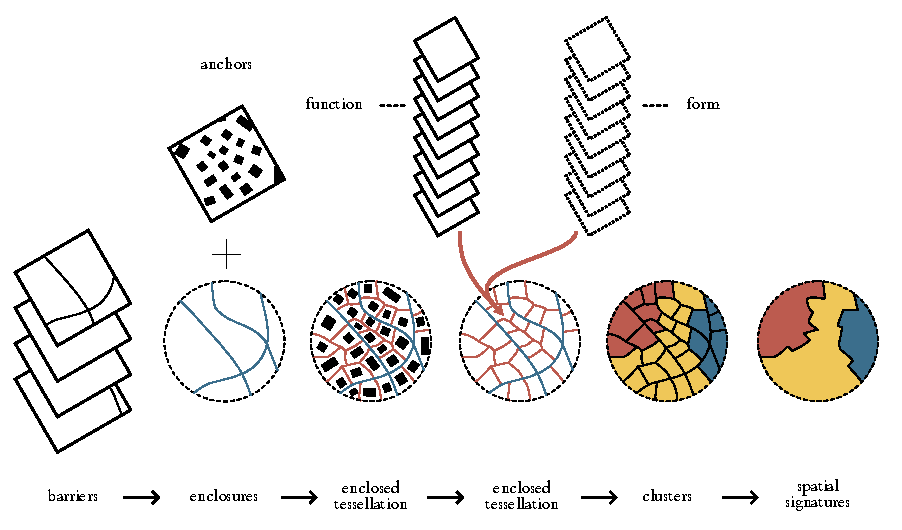
\includegraphics[width=\linewidth]{fig/workflow.pdf}
\caption{Diagram illustrating the sequential steps leading to the delineation of
spatial signatures. From a series of enclosing components, to enclosures,
enclosed tessellation (ET), the addition of form and function characters to ET
cells, and the development of spatial signatures.}
\label{fig:workflow}
\end{figure}


\begin{figure}[ht]
    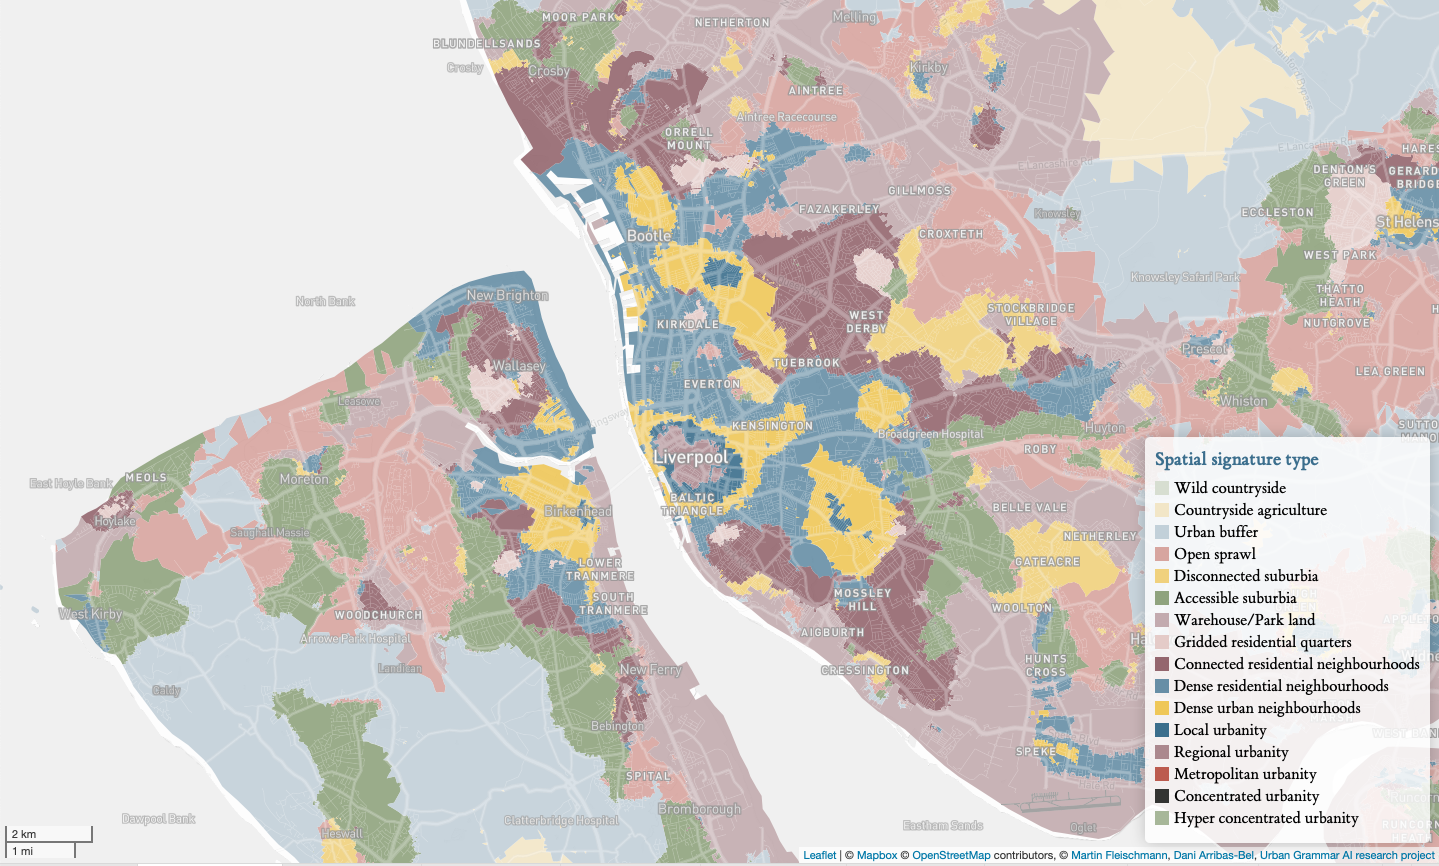
\includegraphics[width=\linewidth]{fig/signatures_map.png}
\caption{Illustration of a classification of spatial signatures in Liverpool and
    Birkenhead area, in the north west of England.}
\label{fig:map}
\end{figure}

\begin{figure}[ht]
    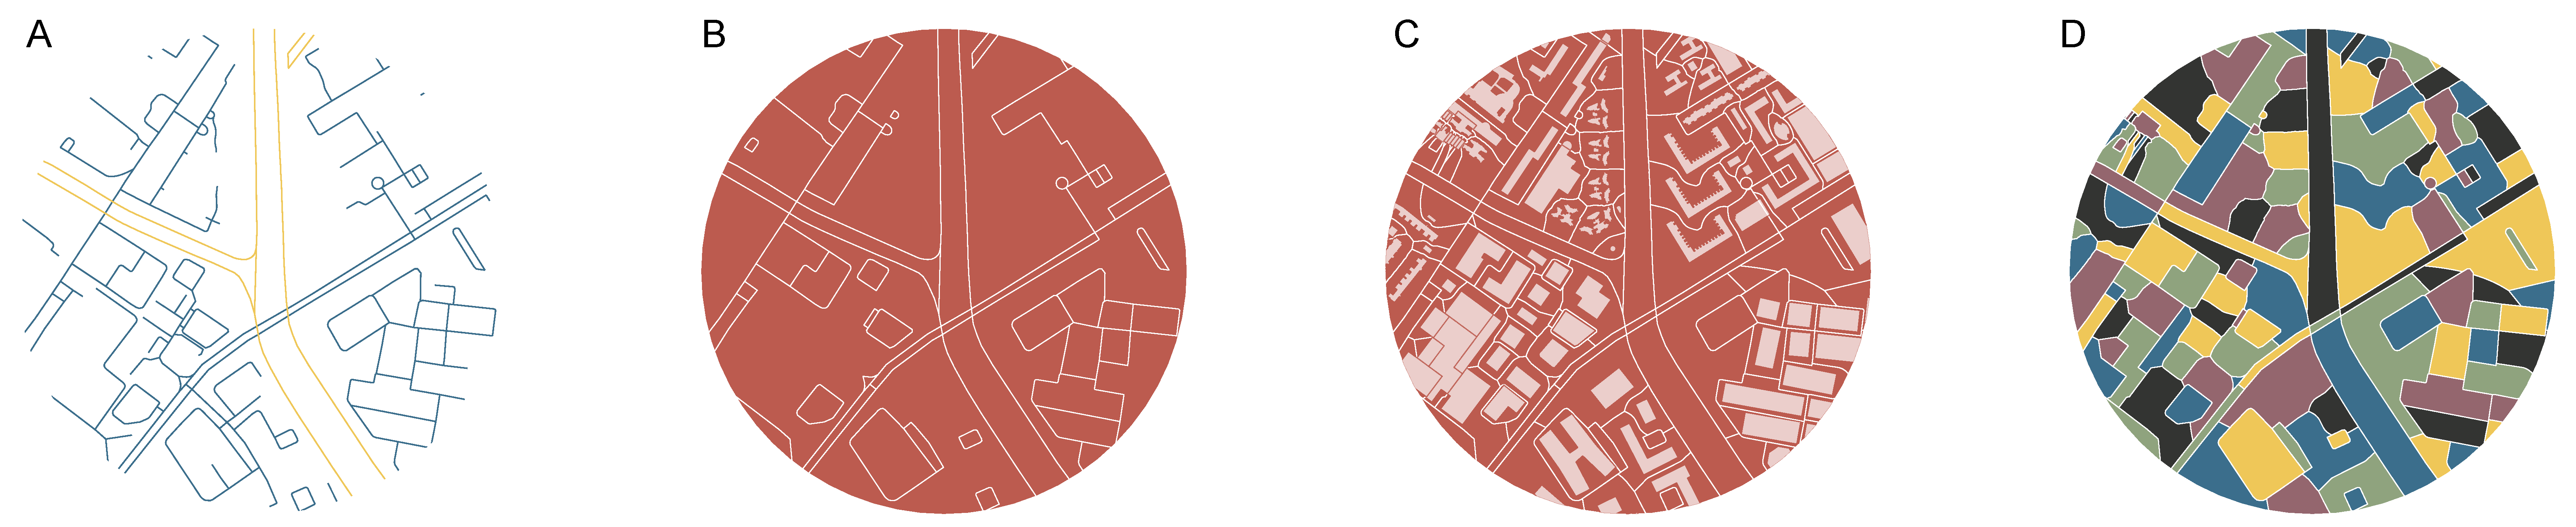
\includegraphics[width=\linewidth]{fig/et_diagram.pdf}
    \caption{Diagram illustrating the sequential steps leading to the delineation of
    enclosed tessellation. From a series of enclosing components, where blue are streets
    and yellow river banks (A), to enclosures (B), incorporation of buildings as anchors
    (C) to final tessellation cells (D).}
    \label{fig:et_diagram}
\end{figure}

\begin{figure}[ht]
    \centering
    \includegraphics[width=.8\linewidth]{fig/cell_context.png}
    \caption{Illustration of a definition of spatial context used to capture the
    distribution of values around each ET cell. For the yellow ET cell in the middle,
    we propose to define a neighbourhood of 10 topological steps on the tessellation
    and weight the importance of each cell within such an area by inverse distance
    between poles of inaccessibility of each cell.}
    \label{fig:context}
\end{figure}

\begin{figure}[ht]
    \centering
    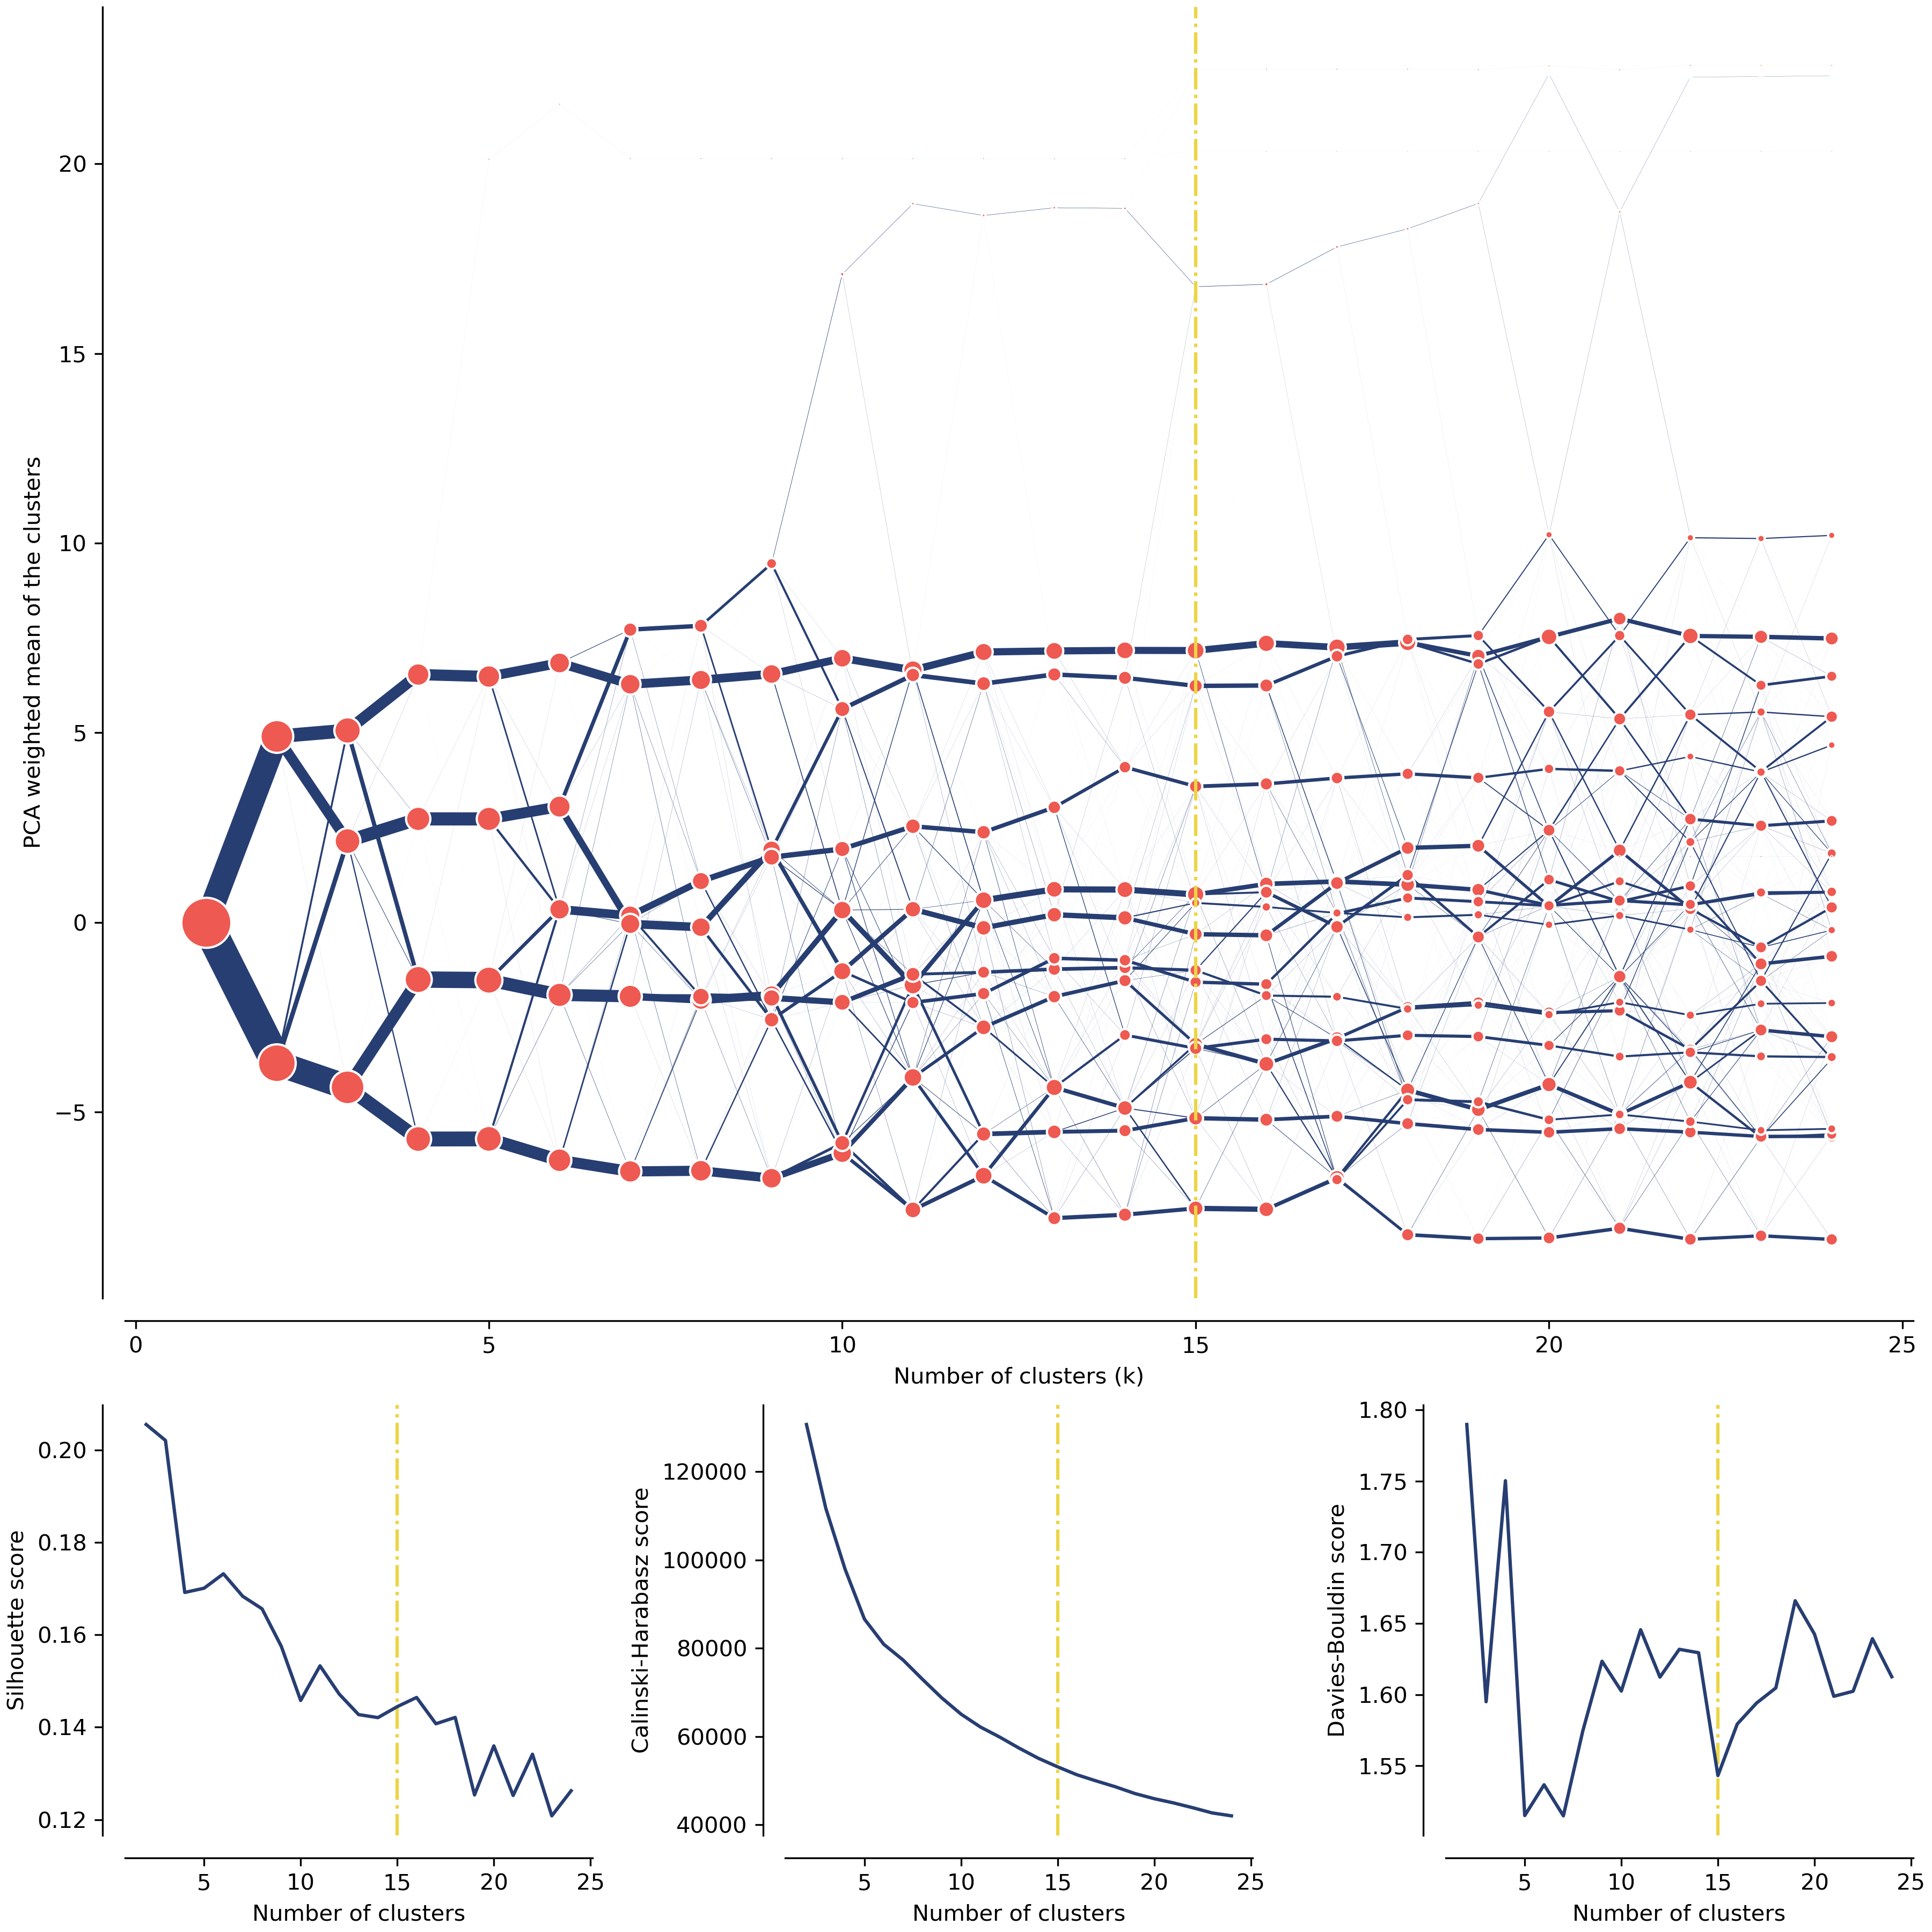
\includegraphics[width=.8\linewidth]{fig/clustergram.png}
    \caption{Clustergram and relevant metrics of a goodness of fit (Silhouette score,
    Calinski-Harabazs score, Davies-Bouldin score) for tested numbers of clusters. The
    clustergram suggest two potential solutions, the very conservative option of 4
    clusters and 10 clusters selected as an optimal result (indicated by a vertical yellow line).}
    \label{fig:clustergram}
\end{figure}

\begin{figure}[ht]
    \centering
    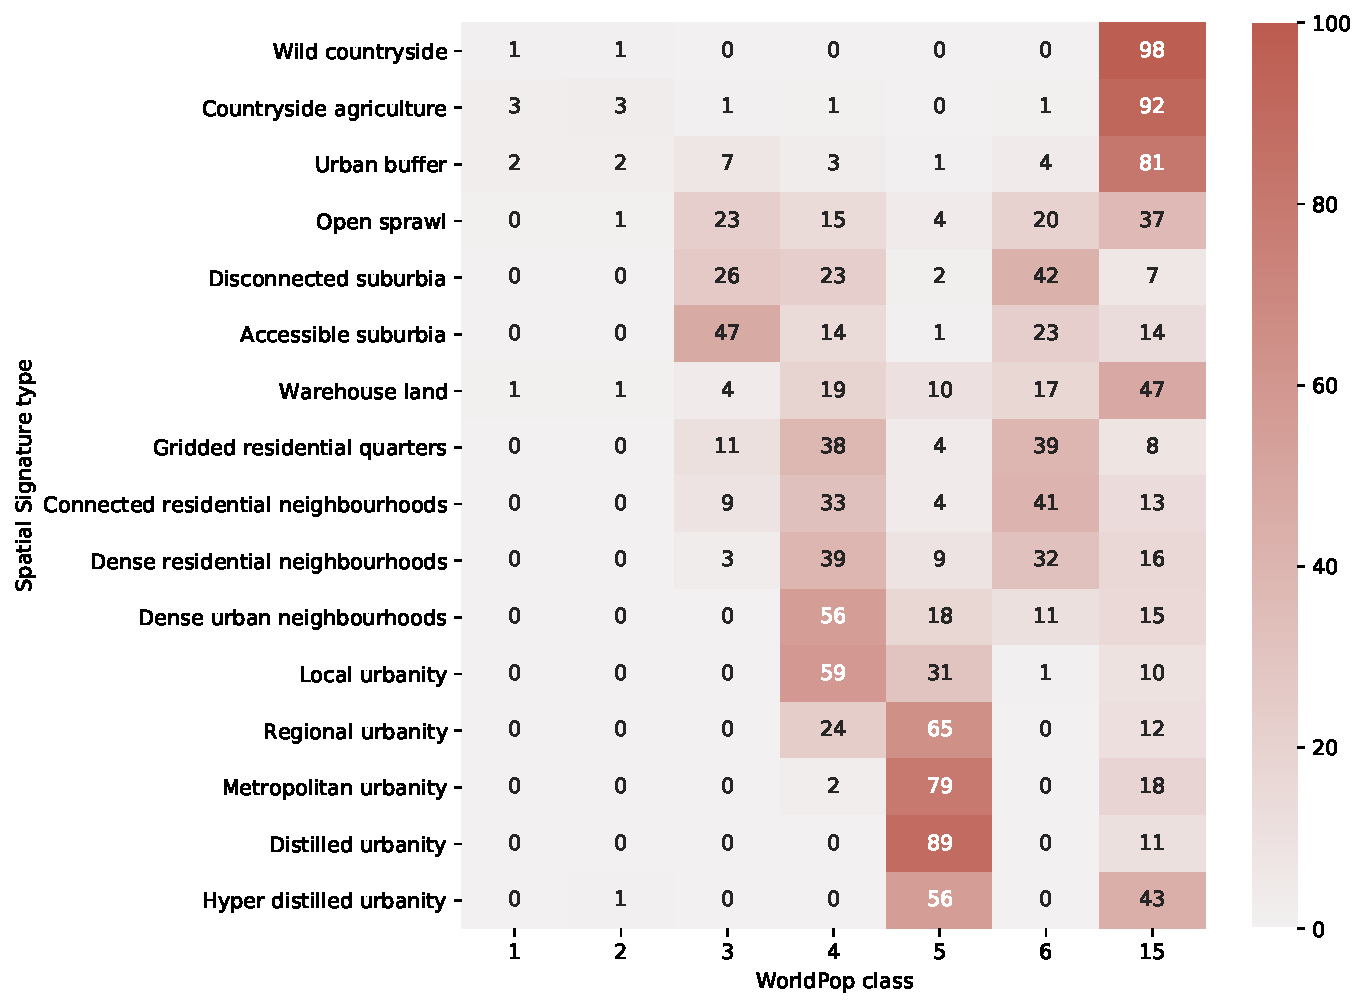
\includegraphics[width=.8\linewidth]{fig/crosstab_worldpop.pdf}
    \caption{Contingency table showing frequencies (in \%) of WorldPop classes within signature types.}
    \label{fig:crosstab_worldpop}
\end{figure}

\begin{figure}[ht]
    \centering
    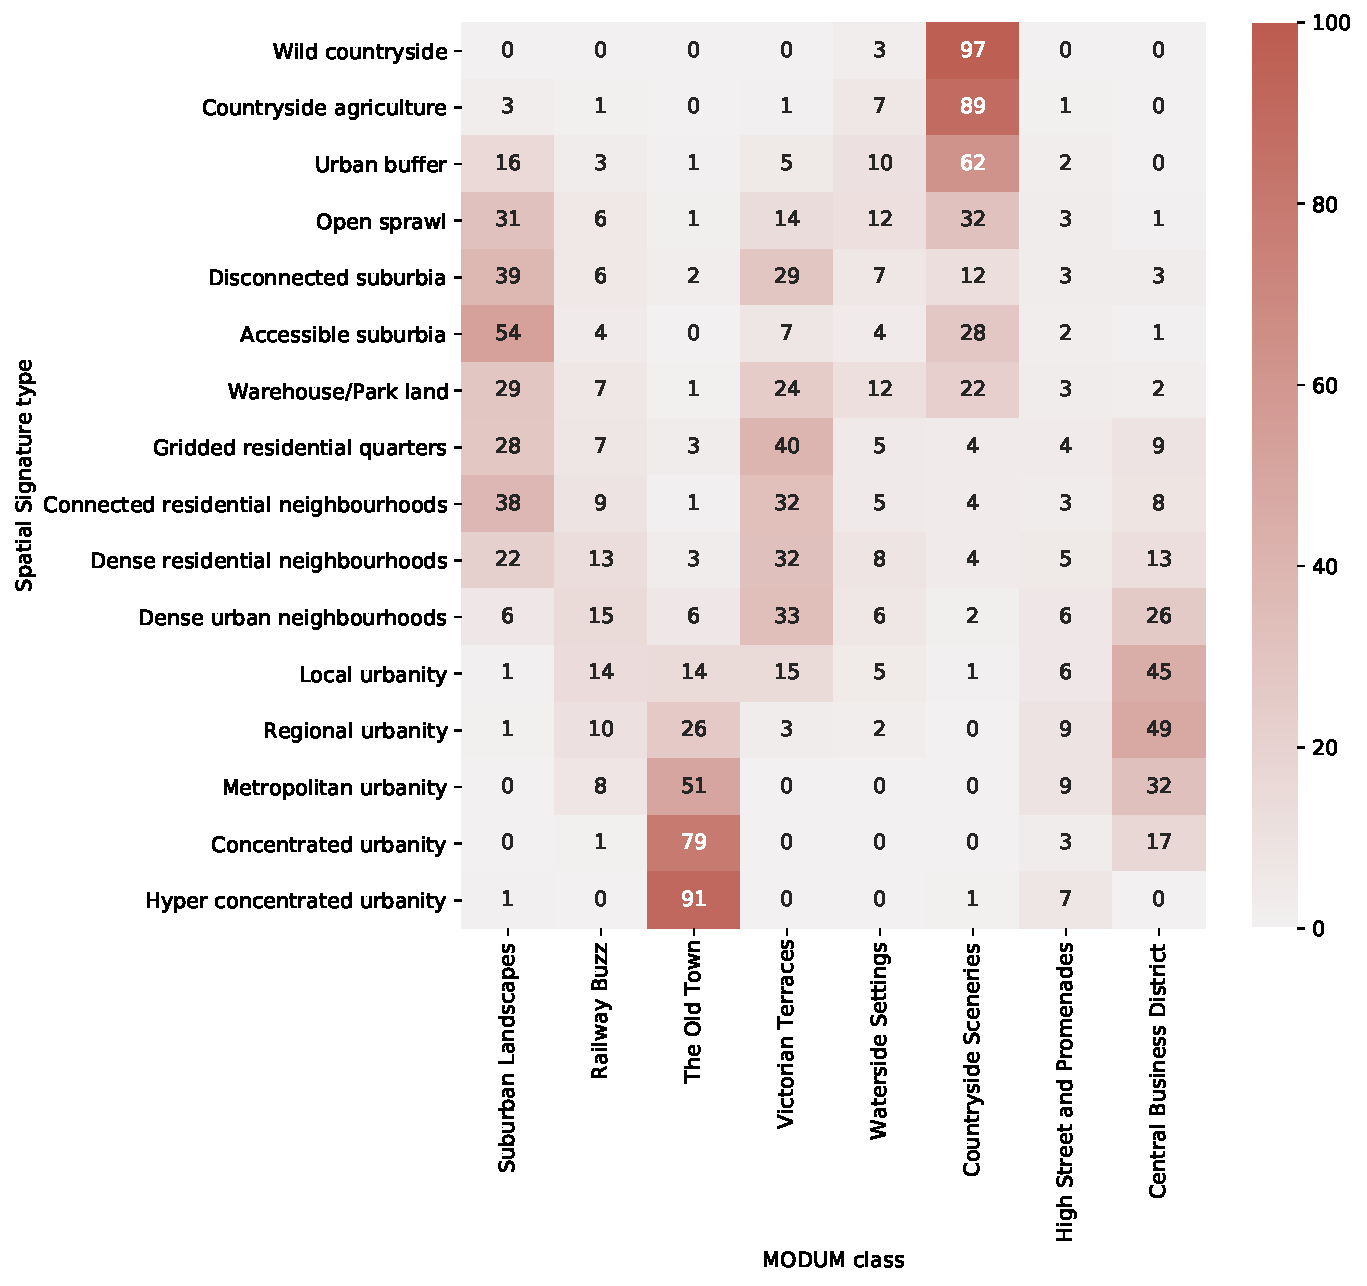
\includegraphics[width=.8\linewidth]{fig/crosstab_modum.pdf}
    \caption{Contingency table showing frequencies (in \%) of MODUM classes within signature types.}
    \label{fig:crosstab_modum}
\end{figure}

\begin{figure}[ht]
    \centering
    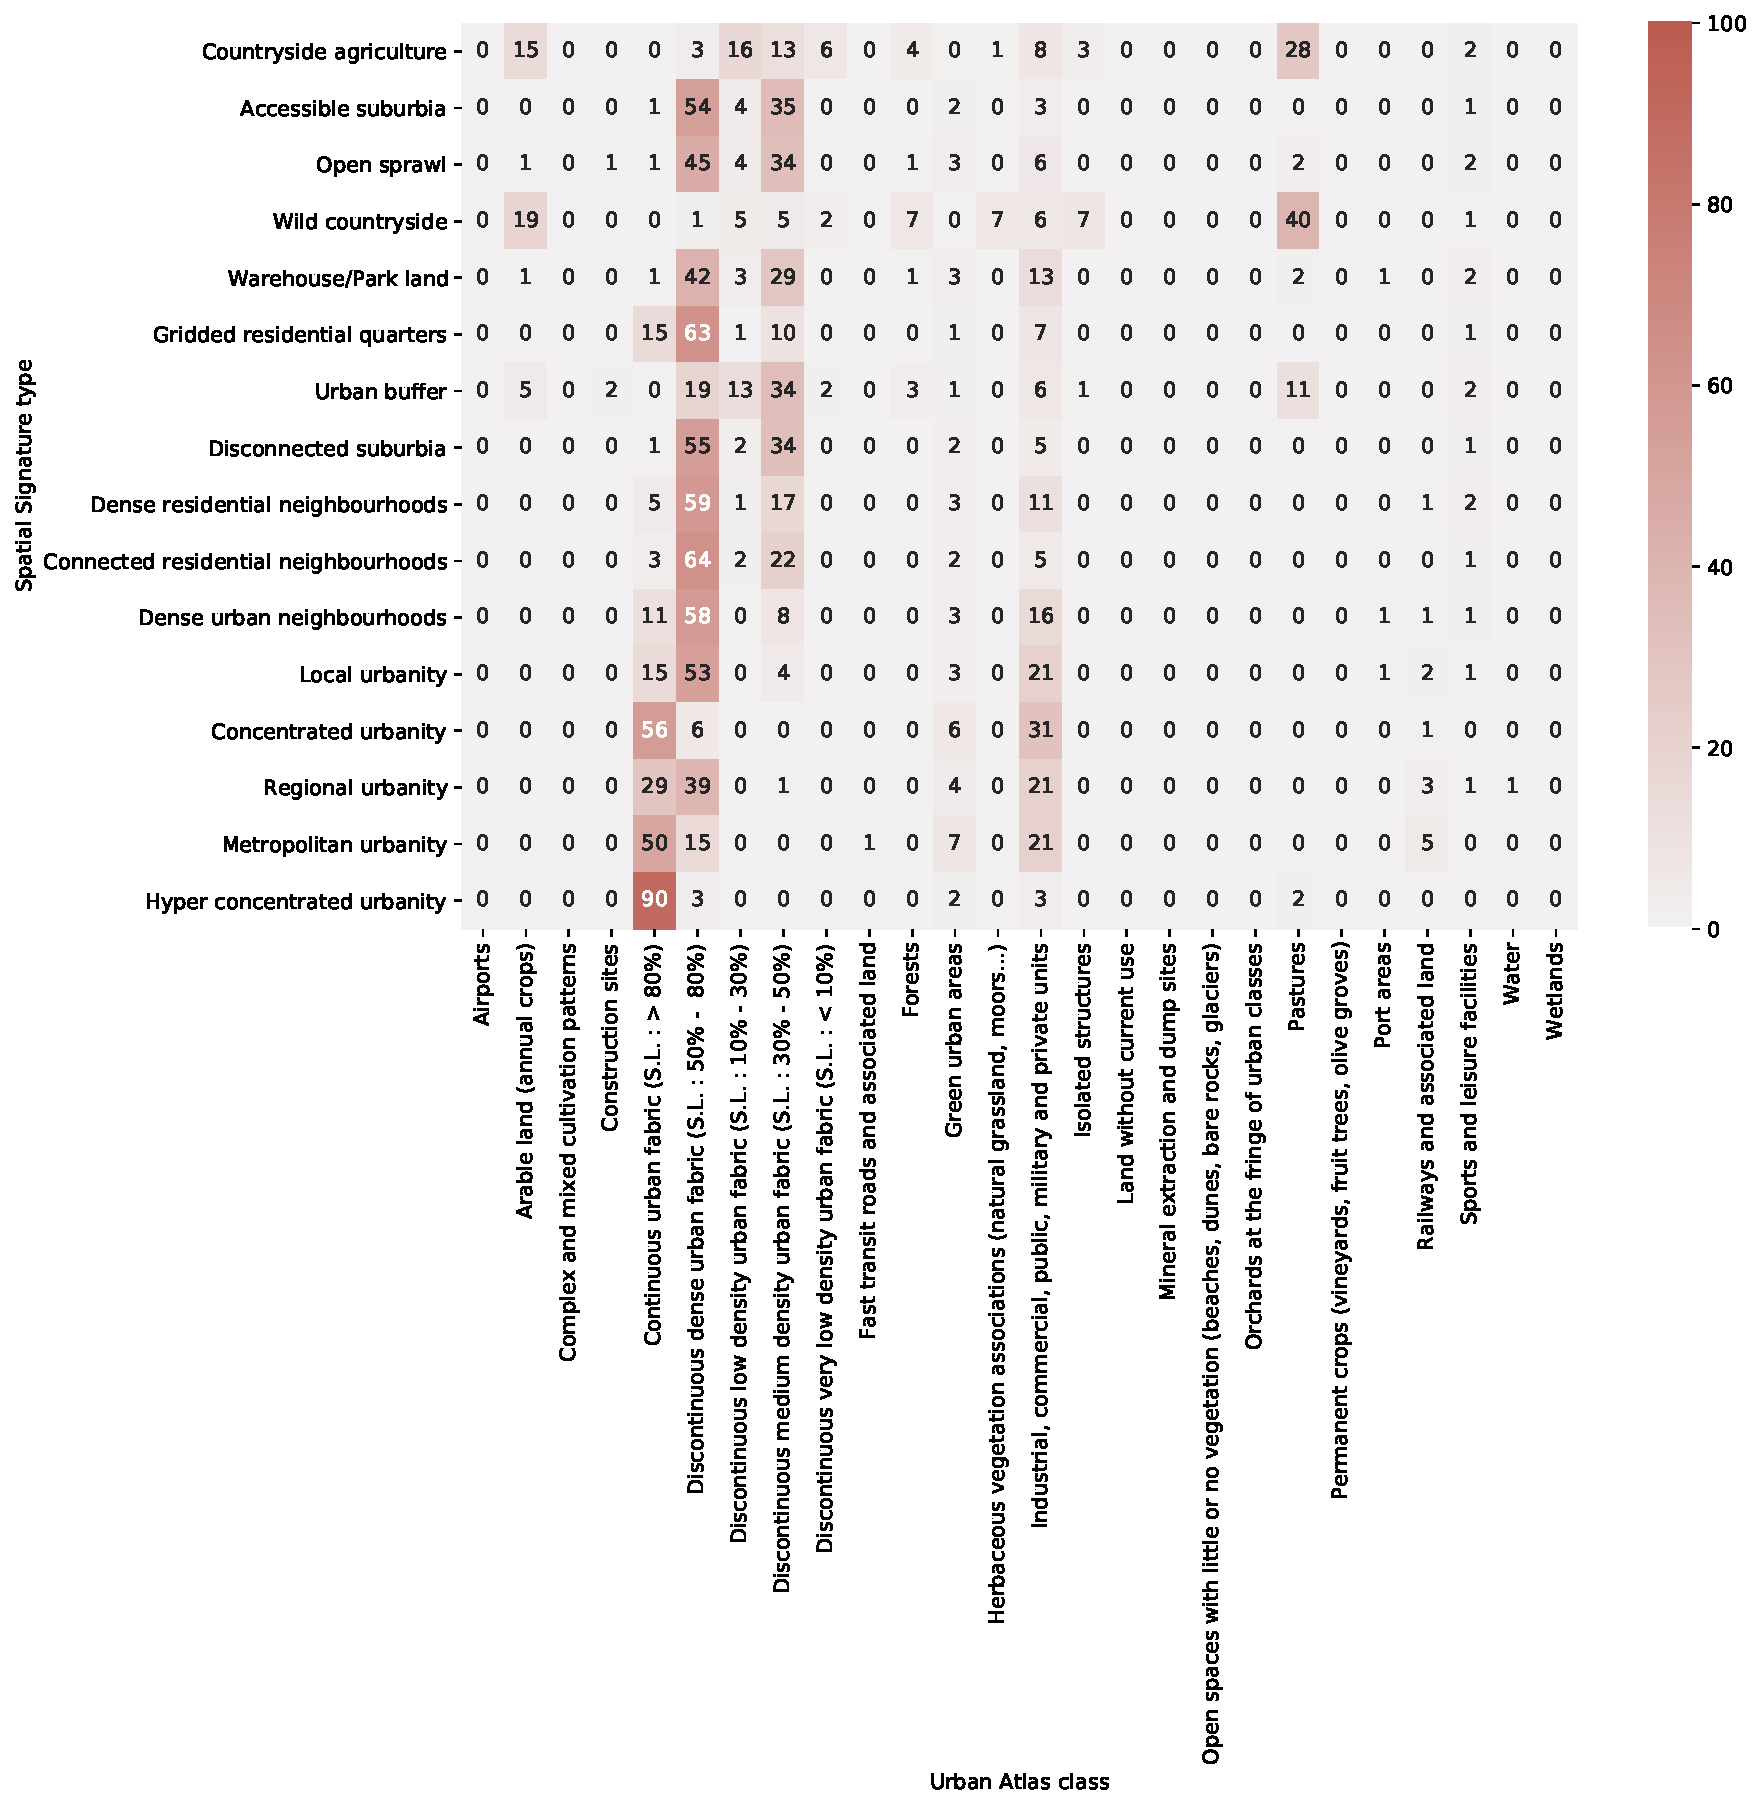
\includegraphics[width=\linewidth]{fig/crosstab_ua.pdf}
    \caption{Contingency table showing frequencies (in \%) of Urban Atlas classes within signature types.}
    \label{fig:crosstab_ua}
\end{figure}

\begin{figure}[ht]
    \centering
    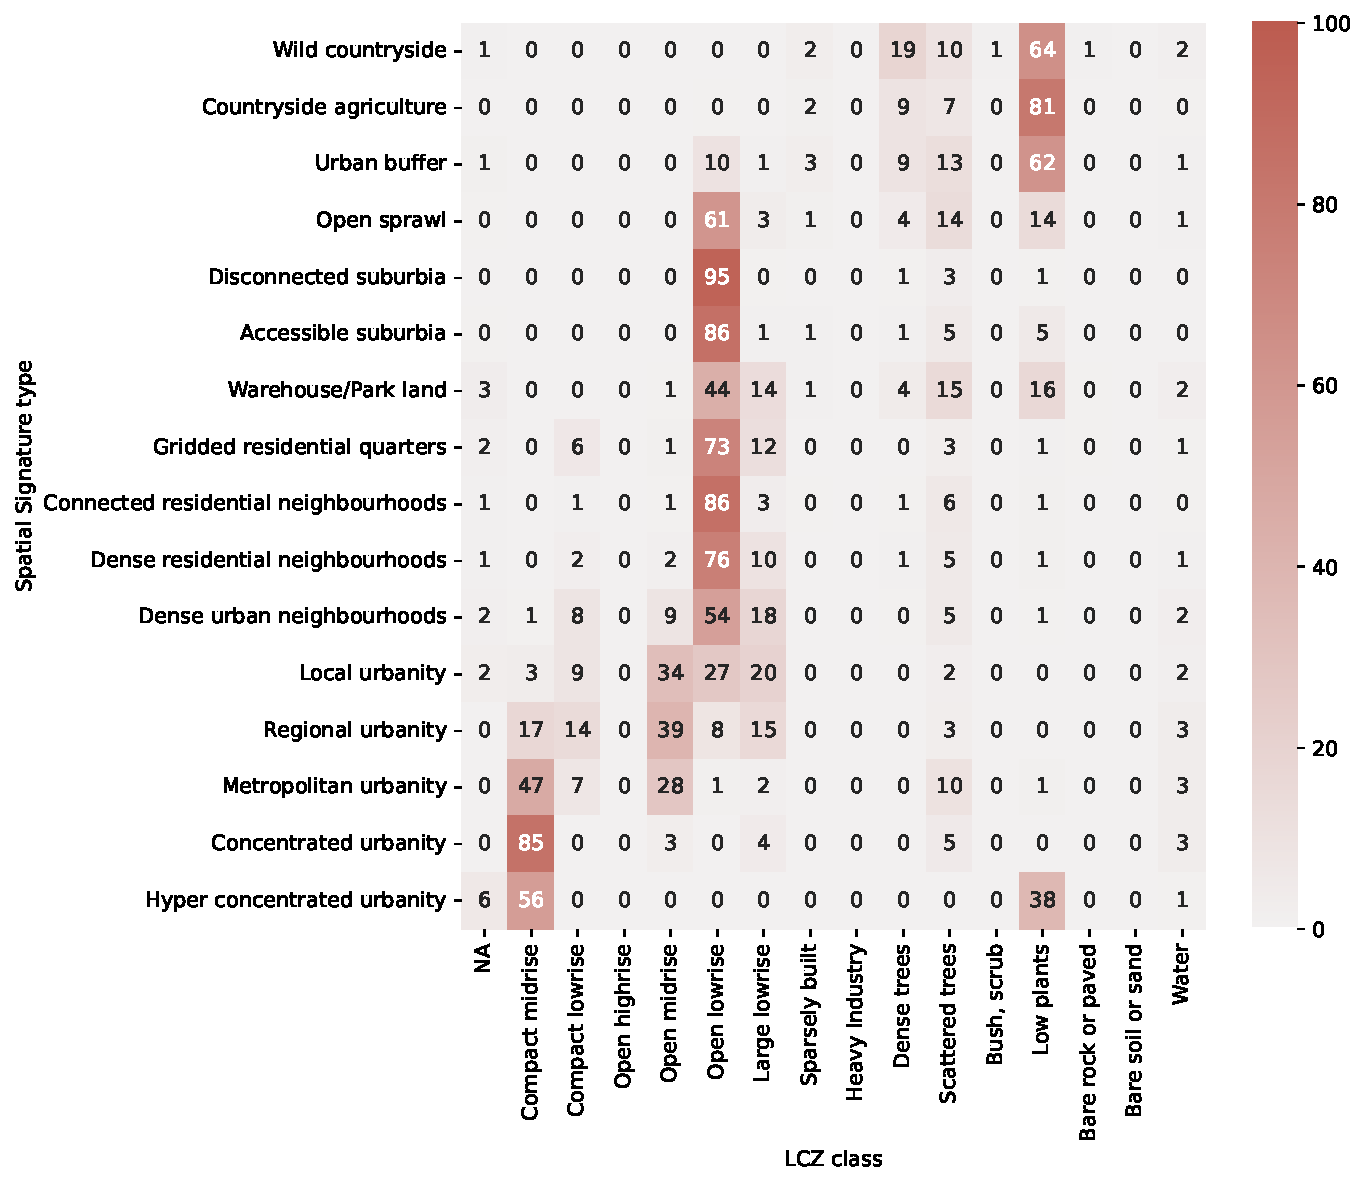
\includegraphics[width=.8\linewidth]{fig/crosstab_lcz.pdf}
    \caption{Contingency table showing frequencies (in \%) of Local Climate Zones within signature types.}
    \label{fig:crosstab_lcz}
\end{figure}

\begin{longtable}{lll}
    \caption{\label{tab:form}Morphometric characters used to
    describe the form component of spatial signatures. For details of the implementation,
    refer to the reproducible Jupyter notebooks available at urbangrammarai.xyz.}\\
    \toprule
                                                character &     category &               reference \\
    \midrule
    \endfirsthead

    \toprule
                                                character &     category &               reference \\
    \midrule
    \endhead
    \midrule
    \multicolumn{3}{r}{{Continued on next page}} \\
    \midrule
    \endfoot

    \bottomrule
    \endlastfoot
                                        area of building &    dimension &    \cite{hallowell2013} \\
                                    perimeter of building &    dimension & \cite{vanderhaegen2017} \\
                            courtyard area of building &    dimension &     \cite{schirmer2015} \\
                        circular compactness of building &        shape & \cite{dibble2019origin} \\
                                    corners of building &        shape &    \cite{steiniger2008} \\
                                squareness of building &        shape &    \cite{steiniger2008} \\
                equivalent rectangular index of building &        shape &    \cite{basaraner2017} \\
                                elongation of building &        shape &    \cite{steiniger2008} \\
        centroid - corner distance deviation of building &        shape &  \cite{fleischmann2021} \\
            centroid - corner mean distance of building &    dimension &     \cite{schirmer2015} \\
                                orientation of building & distribution &     \cite{schirmer2015} \\
                            street alignment of building & distribution &     \cite{schirmer2015} \\
                            cell alignment of building & distribution &  \cite{fleischmann2021} \\
                            longest axis length of ETC &    dimension &  \cite{fleischmann2021} \\
                                            area of ETC &    dimension &     \cite{hamaina2012a} \\
                            circular compactness of ETC &        shape &  \cite{fleischmann2021} \\
                    equivalent rectangular index of ETC &        shape &  \cite{fleischmann2021} \\
                                    orientation of ETC & distribution &  \cite{fleischmann2021} \\
                                covered area ratio of ETC &    intensity &      \cite{hamaina2013} \\
                                length of street segment &    dimension &          \cite{gil2012} \\
                                width of street profile &    dimension &       \cite{araldi2019} \\
                            openness of street profile & distribution &       \cite{araldi2019} \\
                        width deviation of street profile &    diversity &       \cite{araldi2019} \\
                            linearity of street segment &        shape &       \cite{araldi2019} \\
                    area covered by edge-attached ETCs &    dimension &  \cite{fleischmann2021} \\
                    buildings per meter of street segment &    intensity &  \cite{fleischmann2021} \\
                    area covered by node-attached ETCs &    dimension &  \cite{fleischmann2021} \\
                    alignment of neighbouring buildings & distribution &       \cite{hijazi2016} \\
            mean distance between neighbouring buildings & distribution &       \cite{hijazi2016} \\
                    perimeter-weighted neighbours of ETC & distribution &  \cite{fleischmann2021} \\
                    area covered by neighbouring cells &    dimension &  \cite{fleischmann2021} \\
                    reached ETCs by neighbouring segments &    intensity &  \cite{fleischmann2021} \\
                    reached area by neighbouring segments &    dimension &  \cite{fleischmann2021} \\
                                node degree of junction & distribution &       \cite{boeing2018} \\
    mean distance to neighbouring nodes of street network &    dimension &  \cite{fleischmann2021} \\
                            mean inter-building distance & distribution &       \cite{caruso2017} \\
                    weighted reached enclosures of ETC &    intensity &  \cite{fleischmann2021} \\
                reached ETCs by tessellation contiguity &    intensity &  \cite{fleischmann2021} \\
                reached area by tessellation contiguity &    dimension &  \cite{fleischmann2021} \\
                                        area of enclosure &    dimension & \cite{dibble2019origin} \\
                                perimeter of enclosure &    dimension &          \cite{gil2012} \\
                        circular compactness of enclosure &        shape &     \cite{schirmer2015} \\
                equivalent rectangular index of enclosure &        shape &    \cite{basaraner2017} \\
                compactness-weighted axis of enclosure &        shape &   \cite{feliciotti2018} \\
                                orientation of enclosure & distribution &          \cite{gil2012} \\
            perimeter-weighted neighbours of enclosure & distribution &  \cite{fleischmann2021} \\
                        area-weighted ETCs of enclosure &    intensity &  \cite{fleischmann2021} \\
                    local meshedness of street network & connectivity &   \cite{feliciotti2018} \\
                    mean segment length within 3 steps &    dimension &  \cite{fleischmann2021} \\
                local cul-de-sac length of street network &    dimension &  \cite{fleischmann2021} \\
                    reached area by local street network &    dimension &  \cite{fleischmann2021} \\
                    reached ETCs by local street network &    intensity &  \cite{fleischmann2021} \\
                    local node density of street network &    intensity &  \cite{fleischmann2021} \\
        local proportion of cul-de-sacs of street network & connectivity &        \cite{lowry2014} \\
    local proportion of 3-way intersections of street network & connectivity &       \cite{boeing2018} \\
    local proportion of 4-way intersections of street network & connectivity &       \cite{boeing2018} \\
    local degree weighted node density of street network &    intensity & \cite{dibble2019origin} \\
                        local closeness of street network & connectivity &        \cite{porta2006} \\
                    square clustering of street network & connectivity &  \cite{fleischmann2021} \\
\end{longtable}


\begin{longtable}{p{0.25\textwidth}p{0.1\textwidth}p{0.2\textwidth}p{0.15\textwidth}p{0.15\textwidth}}
    \caption{\label{tab:function}Functional characters used to
describe the function component of spatial signatures. For details of the implementation,
refer to the reproducible Jupyter notebooks available at urbangrammarai.xyz.}\\
    \toprule
                                                                                                character &                               data  &                                                                     source  &                    input geometry  &                                transfer method  \\
    \midrule
    \endfirsthead

    \toprule
                                                                                                character &                               data  &                                                                     source  &                    input geometry  &                                transfer method  \\
    \midrule
    \endhead
    \midrule
    \multicolumn{5}{r}{{Continued on next page}} \\
    \midrule
    \endfoot

    \bottomrule
    \endlastfoot
                                                                                                Population &               Population estimates  &           ONS Census Output Area population estimates, Statistics.gov.scot  &      Vector (output area polygon)  &  Building-based dasymetric areal interpolation  \\
                                                                                            Night lights &                       Night Lights  &                                                 VIIRS DNB Nighttime Lights  &                     Raster (500m)  &                               Zonal statistics  \\
                                                    Workplace population [Agriculture, energy and water] &               Workplace population  &    ONS Census Workplace population, Scotland's census Workplace population  &      Vector (output area polygon)  &  Building-based dasymetric areal interpolation  \\
                                                                    Workplace population [Manufacturing] &               Workplace population  &    ONS Census Workplace population, Scotland's census Workplace population  &      Vector (output area polygon)  &  Building-based dasymetric areal interpolation  \\
                                                                    Workplace population [Construction] &               Workplace population  &    ONS Census Workplace population, Scotland's census Workplace population  &      Vector (output area polygon)  &  Building-based dasymetric areal interpolation  \\
                                            Workplace population [Distribution, hotels and restaurants] &               Workplace population  &    ONS Census Workplace population, Scotland's census Workplace population  &      Vector (output area polygon)  &  Building-based dasymetric areal interpolation  \\
                                                        Workplace population [Transport and communication] &               Workplace population  &    ONS Census Workplace population, Scotland's census Workplace population  &      Vector (output area polygon)  &  Building-based dasymetric areal interpolation  \\
                Workplace population [Financial, real estate, professional and administrative activities] &               Workplace population  &    ONS Census Workplace population, Scotland's census Workplace population  &      Vector (output area polygon)  &  Building-based dasymetric areal interpolation  \\
                                        Workplace population [Public administration, education and health] &               Workplace population  &    ONS Census Workplace population, Scotland's census Workplace population  &      Vector (output area polygon)  &  Building-based dasymetric areal interpolation  \\
                                                                            Workplace population [Other] &                  Corine land cover  &                                         Copernicus Land Monitoring Service  &  Vector (land cover zone polygon)  &                            Areal interpolation  \\
                                                                                    Land cover [Airports] &                  Corine land cover  &                                         Copernicus Land Monitoring Service  &  Vector (land cover zone polygon)  &                            Areal interpolation  \\
                                                                    Land cover [Non-irrigated arable land] &                  Corine land cover  &                                         Copernicus Land Monitoring Service  &  Vector (land cover zone polygon)  &                            Areal interpolation  \\
                                                            Land cover [Industrial or commercial units] &                  Corine land cover  &                                         Copernicus Land Monitoring Service  &  Vector (land cover zone polygon)  &                            Areal interpolation  \\
                                                                                Land cover [Salt marshes] &                  Corine land cover  &                                         Copernicus Land Monitoring Service  &  Vector (land cover zone polygon)  &                            Areal interpolation  \\
                                                                                    Land cover [Estuaries] &                  Corine land cover  &                                         Copernicus Land Monitoring Service  &  Vector (land cover zone polygon)  &                            Areal interpolation  \\
                                                                Land cover [Sport and leisure facilities] &                  Corine land cover  &                                         Copernicus Land Monitoring Service  &  Vector (land cover zone polygon)  &                            Areal interpolation  \\
                                                                            Land cover [Green urban areas] &                  Corine land cover  &                                         Copernicus Land Monitoring Service  &  Vector (land cover zone polygon)  &                            Areal interpolation  \\
                                                                Land cover [Discontinuous urban fabric] &                  Corine land cover  &                                         Copernicus Land Monitoring Service  &  Vector (land cover zone polygon)  &                            Areal interpolation  \\
                                                                                    Land cover [Pastures] &                  Corine land cover  &                                         Copernicus Land Monitoring Service  &  Vector (land cover zone polygon)  &                            Areal interpolation  \\
                                                                        Land cover [Broad-leaved forest] &                  Corine land cover  &                                         Copernicus Land Monitoring Service  &  Vector (land cover zone polygon)  &                            Areal interpolation  \\
                                                                    Land cover [Mineral extraction sites] &                  Corine land cover  &                                         Copernicus Land Monitoring Service  &  Vector (land cover zone polygon)  &                            Areal interpolation  \\
                                                                                Land cover [Port areas] &                  Corine land cover  &                                         Copernicus Land Monitoring Service  &  Vector (land cover zone polygon)  &                            Areal interpolation  \\
                                                Land cover [Road and rail networks and associated land] &                  Corine land cover  &                                         Copernicus Land Monitoring Service  &  Vector (land cover zone polygon)  &                            Areal interpolation  \\
                                                                                Land cover [Water bodies] &                  Corine land cover  &                                         Copernicus Land Monitoring Service  &  Vector (land cover zone polygon)  &                            Areal interpolation  \\
    Land cover [Land principally occupied by agriculture, with significant areas of natural vegetation] &                  Corine land cover  &                                         Copernicus Land Monitoring Service  &  Vector (land cover zone polygon)  &                            Areal interpolation  \\
                                                                                Land cover [Mixed forest] &                  Corine land cover  &                                         Copernicus Land Monitoring Service  &  Vector (land cover zone polygon)  &                            Areal interpolation  \\
                                                                                    Land cover [Peat bogs] &                  Corine land cover  &                                         Copernicus Land Monitoring Service  &  Vector (land cover zone polygon)  &                            Areal interpolation  \\
                                                                        Land cover [Natural grasslands] &                  Corine land cover  &                                         Copernicus Land Monitoring Service  &  Vector (land cover zone polygon)  &                            Areal interpolation  \\
                                                                        Land cover [Moors and heathland] &                  Corine land cover  &                                         Copernicus Land Monitoring Service  &  Vector (land cover zone polygon)  &                            Areal interpolation  \\
                                                                Land cover [Transitional woodland-shrub] &                  Corine land cover  &                                         Copernicus Land Monitoring Service  &  Vector (land cover zone polygon)  &                            Areal interpolation  \\
                                                                    Land cover [Continuous urban fabric] &                  Corine land cover  &                                         Copernicus Land Monitoring Service  &  Vector (land cover zone polygon)  &                            Areal interpolation  \\
                                                                            Land cover [Intertidal flats] &                  Corine land cover  &                                         Copernicus Land Monitoring Service  &  Vector (land cover zone polygon)  &                            Areal interpolation  \\
                                                                                Land cover [Sea and ocean] &                  Corine land cover  &                                         Copernicus Land Monitoring Service  &  Vector (land cover zone polygon)  &                            Areal interpolation  \\
                                                                            Land cover [Coniferous forest] &                  Corine land cover  &                                         Copernicus Land Monitoring Service  &  Vector (land cover zone polygon)  &                            Areal interpolation  \\
                                                                        Land cover [Construction sites] &                  Corine land cover  &                                         Copernicus Land Monitoring Service  &  Vector (land cover zone polygon)  &                            Areal interpolation  \\
                                                                    Land cover [Sparsely vegetated areas] &                  Corine land cover  &                                         Copernicus Land Monitoring Service  &  Vector (land cover zone polygon)  &                            Areal interpolation  \\
                                                                                Land cover [Bare rocks] &                  Corine land cover  &                                         Copernicus Land Monitoring Service  &  Vector (land cover zone polygon)  &                            Areal interpolation  \\
                                                                            Land cover [Inland marshes] &                  Corine land cover  &                                         Copernicus Land Monitoring Service  &  Vector (land cover zone polygon)  &                            Areal interpolation  \\
                                                                                Land cover [Dump sites] &                  Corine land cover  &                                         Copernicus Land Monitoring Service  &  Vector (land cover zone polygon)  &                            Areal interpolation  \\
                                                            Land cover [Fruit trees and berry plantations] &                  Corine land cover  &                                         Copernicus Land Monitoring Service  &  Vector (land cover zone polygon)  &                            Areal interpolation  \\
                                                                Land cover [Complex cultivation patterns] &                  Corine land cover  &                                         Copernicus Land Monitoring Service  &  Vector (land cover zone polygon)  &                            Areal interpolation  \\
                                                                        Land cover [Beaches, dunes, sands] &                  Corine land cover  &                                         Copernicus Land Monitoring Service  &  Vector (land cover zone polygon)  &                            Areal interpolation  \\
                                                                                Land cover [Water courses] &                  Corine land cover  &                                         Copernicus Land Monitoring Service  &  Vector (land cover zone polygon)  &                            Areal interpolation  \\
                                                                                Land cover [Burnt areas] &                  Corine land cover  &                                         Copernicus Land Monitoring Service  &  Vector (land cover zone polygon)  &                            Areal interpolation  \\
                                                                        Land cover [Agro-forestry areas] &                  Corine land cover  &                                         Copernicus Land Monitoring Service  &  Vector (land cover zone polygon)  &                            Areal interpolation  \\
                                                                            Land cover [Coastal lagoons] &                  Corine land cover  &                                         Copernicus Land Monitoring Service  &  Vector (land cover zone polygon)  &                            Areal interpolation  \\
                                                                                                    NDVI &                               NDVI  &                                                    GHS-composite-S2 R2020A  &                      Raster (10m)  &                               Zonal statistics  \\
                                                                        Supermarkets [distance to nearest] &         Retail POIs (supermarkets)  &                                                                   Geolytix  &                    Vector (point)  &              Network-constrained accessibility  \\
                                                                        Supermarkets [counts within 1200m] &         Retail POIs (supermarkets)  &                                                                   Geolytix  &                    Vector (point)  &              Network-constrained accessibility  \\
                                                                    Listed buildings [distance to nearest] &                   Listed Buildings  &  Historic England, Historic Environment Scotland, Lle Geo-Portal for Wales  &                    Vector (point)  &              Network-constrained accessibility  \\
                                                                    Listed buildings [counts within 1200m] &                   Listed Buildings  &  Historic England, Historic Environment Scotland, Lle Geo-Portal for Wales  &                    Vector (point)  &              Network-constrained accessibility  \\
                                                                        FHRS points [distance to nearest] & Food Hygiene Rating Scheme Ratings  &                                                                 CDRC.ac.uk  &                    Vector (point)  &              Network-constrained accessibility  \\
                                                                        FHRS points [counts within 1200m] & Food Hygiene Rating Scheme Ratings  &                                                                 CDRC.ac.uk  &                    Vector (point)  &              Network-constrained accessibility  \\
                                                                    Cultural venues [distance to nearest] &        Culture (theatres, cinemas)  &                                                              OpenStreetMap  &                    Vector (point)  &              Network-constrained accessibility  \\
                                                                    Cultural venues [counts within 1200m] &        Culture (theatres, cinemas)  &                                                              OpenStreetMap  &                    Vector (point)  &              Network-constrained accessibility  \\
                                                                        Water bodies [distance to nearest] &                       Water bodies  &                                                           OS OpenMap Local  &       Vector (water body polygon)  &                        Euclidean accessibility  \\
                                                                    Retail centres [distance to nearest] &                     Retail centres  &                                                                 CDRC.ac.uk  &    Vector (retail centre polygon)  &                        Euclidean accessibility  \\
\end{longtable}

\tiny
    \begin{longtable}{p{0.1\textwidth}p{0.035\textwidth}p{0.035\textwidth}p{0.035\textwidth}p{0.035\textwidth}p{0.035\textwidth}p{0.035\textwidth}p{0.035\textwidth}p{0.035\textwidth}p{0.035\textwidth}p{0.035\textwidth}p{0.035\textwidth}p{0.035\textwidth}p{0.035\textwidth}p{0.035\textwidth}p{0.035\textwidth}p{0.035\textwidth}}
        \caption{\label{tab:port}Numerical portraits characterising each signature type. Each value is computed as a mean of values of all ETCs within the type.}\\

        \toprule
        type &  Accessible suburbia &  Connected residential neighbourhoods &  Countryside agriculture &  Dense residential neighbourhoods &  Dense urban neighbourhoods &  Disconnected suburbia &  Concentrated urbanity &  Gridded residential quarters &  Hyper concentrated urbanity &  Local urbanity &  Metropolitan urbanity &  Open sprawl &  Regional urbanity &  Urban buffer &  Warehouse / Park land &  Wild countryside \\
        \midrule
        \endfirsthead

        \toprule
        type &  Accessible suburbia &  Connected residential neighbourhoods &  Countryside agriculture &  Dense residential neighbourhoods &  Dense urban neighbourhoods &  Disconnected suburbia &  Concentrated urbanity &  Gridded residential quarters &  Hyper concentrated urbanity &  Local urbanity &  Metropolitan urbanity &  Open sprawl &  Regional urbanity &  Urban buffer &  Warehouse / Park land &  Wild countryside \\
        \midrule
        \endhead
        \midrule
        \multicolumn{17}{r}{{Continued on next page}} \\
        \midrule
        \endfoot

        \bottomrule
        \endlastfoot

        area of building                                                                                    &               176.95 &                                272.52 &                   204.10 &                            375.60 &                      588.36 &                 212.71 &                3713.38 &                        283.89 &                      3358.10 &          823.35 &                2413.94 &       226.72 &            1480.26 &        209.42 &               393.22 &            209.86 \\
        perimeter of building                                                                               &                53.90 &                                 69.12 &                    56.05 &                             80.56 &                      107.36 &                  61.63 &                 376.30 &                         69.67 &                       330.82 &          135.54 &                 283.94 &        59.64 &             195.98 &         55.94 &                75.68 &             57.12 \\
        courtyard area of building                                                                          &                 0.48 &                                  1.07 &                     0.51 &                              2.13 &                        5.03 &                   0.52 &                 159.09 &                          0.75 &                        90.82 &           12.67 &                 118.95 &         0.90 &              43.19 &          0.74 &                 3.26 &              0.22 \\
        circular compactness of building                                                                    &                 0.53 &                                  0.48 &                     0.51 &                              0.47 &                        0.44 &                   0.49 &                   0.43 &                          0.49 &                         0.45 &            0.41 &                   0.40 &         0.52 &               0.39 &          0.52 &                 0.47 &              0.50 \\
        corners of building                                                                                 &                 4.25 &                                  4.45 &                     4.37 &                              4.69 &                        5.21 &                   4.35 &                  12.48 &                          4.51 &                         9.27 &            6.01 &                   9.72 &         4.37 &               7.78 &          4.34 &                 4.56 &              4.38 \\
        squareness of building                                                                              &                 0.78 &                                  1.47 &                     0.81 &                              1.86 &                        3.28 &                   1.02 &                  18.59 &                          1.66 &                        22.51 &            5.07 &                  12.41 &         0.99 &               8.84 &          0.86 &                 1.35 &              0.71 \\
        equivalent rectangular index of building                                                            &                 0.99 &                                  0.98 &                     0.98 &                              0.97 &                        0.95 &                   0.98 &                   0.78 &                          0.98 &                         0.80 &            0.92 &                   0.82 &         0.98 &               0.87 &          0.98 &                 0.98 &              0.98 \\
        elongation of building                                                                              &                 0.64 &                                  0.56 &                     0.60 &                              0.56 &                        0.52 &                   0.57 &                   0.59 &                          0.58 &                         0.62 &            0.51 &                   0.53 &         0.62 &               0.51 &          0.63 &                 0.54 &              0.59 \\
        centroid - corner mean distance of building                                                         &                 9.60 &                                 12.41 &                     9.79 &                             13.96 &                       18.00 &                  11.11 &                  35.93 &                         12.41 &                        37.22 &           20.71 &                  29.68 &        10.49 &              25.25 &          9.81 &                13.20 &              9.95 \\
        centroid - corner distance deviation of building                                                    &                 0.36 &                                  0.71 &                     0.56 &                              1.07 &                        1.88 &                   0.54 &                   9.03 &                          0.80 &                         7.70 &            2.98 &                   6.78 &         0.55 &               4.98 &          0.49 &                 0.88 &              0.60 \\
        orientation of building                                                                             &                19.56 &                                 25.50 &                    20.57 &                             16.41 &                       20.64 &                  26.39 &                  20.32 &                         23.13 &                        26.26 &           20.78 &                  22.30 &        20.21 &              21.82 &         21.10 &                23.30 &             21.86 \\
        longest axis length of ETC                                                                          &                50.84 &                                 57.72 &                   220.30 &                             64.46 &                       73.56 &                  53.55 &                 112.12 &                         52.89 &                       126.58 &           80.14 &                 100.52 &        60.97 &              91.91 &        105.16 &                78.67 &            449.71 \\
        area of ETC                                                                                         &              1147.25 &                               1517.81 &                 31193.48 &                           1917.31 &                     2410.32 &                1259.03 &                5708.23 &                       1251.54 &                      8654.32 &         2696.40 &                4442.21 &      2000.37 &            3535.28 &       8658.83 &              3520.84 &         155623.92 \\
        circular compactness of ETC                                                                         &                 0.47 &                                  0.48 &                     0.38 &                              0.48 &                        0.47 &                   0.49 &                   0.46 &                          0.48 &                         0.47 &            0.46 &                   0.42 &         0.47 &               0.44 &          0.44 &                 0.46 &              0.35 \\
        equivalent rectangular index of ETC                                                                 &                 0.97 &                                  0.97 &                     0.93 &                              0.96 &                        0.96 &                   0.97 &                   0.94 &                          0.97 &                         0.95 &            0.95 &                   0.93 &         0.97 &               0.94 &          0.95 &                 0.96 &              0.91 \\
        orientation of ETC                                                                                  &                20.40 &                                 24.94 &                    21.92 &                             17.77 &                       21.07 &                  25.28 &                  20.37 &                         23.06 &                        25.96 &           21.22 &                  22.38 &        21.07 &              21.88 &         21.86 &                23.27 &             22.51 \\
        covered area ratio of ETC                                                                           &                 0.19 &                                  0.20 &                     0.07 &                              0.52 &                        0.27 &                   0.22 &                   0.91 &                          0.23 &                         0.61 &            0.60 &                   4.85 &         0.18 &            1122.51 &          0.14 &                 0.18 &              0.04 \\
        cell alignment of building                                                                          &                 7.38 &                                  6.12 &                    11.49 &                              6.52 &                        5.61 &                   8.08 &                   4.43 &                          5.48 &                         2.72 &            5.64 &                   4.86 &         8.64 &               5.25 &          9.76 &                 8.03 &             12.55 \\
        alignment of neighbouring buildings                                                                 &                 5.31 &                                  5.36 &                     8.45 &                              5.39 &                        5.17 &                   5.67 &                   5.95 &                          4.93 &                         6.55 &            5.67 &                   6.37 &         6.48 &               6.27 &          7.06 &                 6.06 &             10.05 \\
        mean distance between neighbouring buildings                                                        &                17.82 &                                 19.17 &                   111.38 &                             20.84 &                       21.13 &                  18.63 &                  18.96 &                         16.48 &                        22.95 &           20.62 &                  22.33 &        22.13 &              20.94 &         45.37 &                28.71 &            238.45 \\
        perimeter-weighted neighbours of ETC                                                                &                 0.04 &                                  0.04 &                     0.02 &                              0.04 &                        0.07 &                   0.05 &                   0.03 &                          0.04 &                         0.04 &            0.11 &                   0.04 &         0.06 &               7.46 &          0.13 &                 0.04 &              0.01 \\
        area covered by neighbouring cells                                                                  &              8620.11 &                              11990.46 &                277883.95 &                          15619.36 &                    20375.37 &                9503.57 &               52023.10 &                       9962.17 &                     61122.40 &        22892.04 &               39665.51 &     16780.98 &           31594.99 &      76942.43 &             31956.96 &        1485709.28 \\
        weighted reached enclosures of ETC                                                                  &                 0.00 &                                  0.00 &                     0.00 &                              0.00 &                        0.00 &                   0.00 &                   0.00 &                          0.00 &                         0.00 &            0.00 &                   0.00 &         0.00 &               0.00 &          0.00 &                 0.00 &              0.00 \\
        mean inter-building distance                                                                        &                21.97 &                                 24.07 &                   167.60 &                             26.48 &                       27.37 &                  22.03 &                  22.73 &                         21.34 &                        23.74 &           26.28 &                  26.99 &        28.94 &              26.32 &         67.27 &                40.97 &            367.72 \\
        width of street profile                                                                             &                28.38 &                                 26.84 &                    32.84 &                             26.29 &                       24.84 &                  27.65 &                  19.47 &                         24.27 &                        17.47 &           24.56 &                  22.61 &        28.59 &              23.44 &         31.00 &                30.85 &             34.31 \\
        width deviation of street profile                                                                   &                 3.30 &                                  3.27 &                     3.91 &                              3.50 &                        3.45 &                   3.71 &                   3.29 &                          3.87 &                         2.85 &            3.60 &                   3.50 &         3.74 &               3.62 &          3.76 &                 3.26 &              3.41 \\
        openness of street profile                                                                          &                 0.42 &                                  0.41 &                     0.83 &                              0.43 &                        0.41 &                   0.44 &                   0.28 &                          0.38 &                         0.22 &            0.41 &                   0.37 &         0.48 &               0.39 &          0.62 &                 0.53 &              0.92 \\
        length of street segment                                                                            &               187.61 &                                162.45 &                   574.25 &                            153.66 &                      151.58 &                 150.53 &                 108.90 &                        126.02 &                        93.90 &          143.14 &                 123.30 &       183.43 &             132.18 &        333.77 &               220.94 &            842.79 \\
        linearity of street segment                                                                         &                 0.93 &                                  0.94 &                     0.93 &                              0.92 &                        0.93 &                   0.92 &                   0.94 &                          0.94 &                         0.97 &            0.92 &                   0.93 &         0.90 &               0.92 &          0.91 &                 0.91 &              0.91 \\
        mean segment length within 3 steps                                                                  &              2327.31 &                               2374.39 &                  5884.25 &                           1992.44 &                     2113.58 &                1707.52 &                1944.94 &                       1950.07 &                      2057.70 &         2011.42 &                2112.12 &      1862.02 &            2034.72 &       3170.78 &              2339.74 &           8062.03 \\
        node degree of junction                                                                             &                 2.87 &                                  3.00 &                     2.78 &                              2.89 &                        2.94 &                   2.68 &                   3.12 &                          3.04 &                         3.33 &            2.94 &                   3.14 &         2.68 &               3.01 &          2.70 &                 2.77 &              2.69 \\
        local meshedness of street network                                                                  &                 0.08 &                                  0.11 &                     0.06 &                              0.10 &                        0.11 &                   0.05 &                   0.14 &                          0.13 &                         0.17 &            0.11 &                   0.14 &         0.06 &               0.12 &          0.05 &                 0.08 &              0.05 \\
        local proportion of 3-way intersections of street network                                           &                 0.74 &                                  0.74 &                     0.72 &                              0.74 &                        0.74 &                   0.71 &                   0.76 &                          0.72 &                         0.70 &            0.75 &                   0.75 &         0.71 &               0.76 &          0.71 &                 0.75 &              0.68 \\
        local proportion of 4-way intersections of street network                                           &                 0.07 &                                  0.12 &                     0.04 &                              0.09 &                        0.11 &                   0.04 &                   0.15 &                          0.16 &                         0.23 &            0.11 &                   0.17 &         0.04 &               0.13 &          0.04 &                 0.05 &              0.04 \\
        local proportion of cul-de-sacs of street network                                                   &                 0.19 &                                  0.14 &                     0.24 &                              0.17 &                        0.14 &                   0.25 &                   0.09 &                          0.12 &                         0.06 &            0.14 &                   0.08 &         0.25 &               0.11 &          0.25 &                 0.20 &              0.28 \\
        local closeness of street network                                                                   &                 0.00 &                                  0.00 &                     0.00 &                              0.00 &                        0.00 &                   0.00 &                   0.00 &                          0.00 &                         0.00 &            0.00 &                   0.00 &         0.00 &               0.00 &          0.00 &                 0.00 &              0.00 \\
        local cul-de-sac length of street network                                                           &               228.58 &                                163.78 &                   636.07 &                            196.63 &                      170.89 &                 275.96 &                  84.41 &                        133.13 &                        75.11 &          167.72 &                  79.56 &       288.26 &             128.76 &        408.67 &               253.49 &           1186.52 \\
        square clustering of street network                                                                 &                 0.03 &                                  0.04 &                     0.01 &                              0.03 &                        0.04 &                   0.01 &                   0.03 &                          0.04 &                         0.04 &            0.03 &                   0.04 &         0.02 &               0.03 &          0.02 &                 0.03 &              0.01 \\
        mean distance to neighbouring nodes of street network                                               &               132.49 &                                118.06 &                   373.74 &                            112.48 &                      111.55 &                 111.69 &                  86.38 &                         92.19 &                        81.24 &          106.90 &                  93.66 &       129.03 &              99.79 &        212.34 &               150.43 &            601.60 \\
        local node density of street network                                                                &                 0.02 &                                  0.02 &                     0.01 &                              0.02 &                        0.02 &                   0.03 &                   0.02 &                          0.02 &                         0.02 &            0.02 &                   0.02 &         0.03 &               0.02 &          0.02 &                 0.02 &              0.01 \\
        local degree weighted node density of street network                                                &                 0.03 &                                  0.03 &                     0.02 &                              0.04 &                        0.04 &                   0.04 &                   0.04 &                          0.04 &                         0.04 &            0.04 &                   0.04 &         0.04 &               0.04 &          0.03 &                 0.03 &              0.01 \\
        street alignment of building                                                                        &                 8.73 &                                  7.53 &                    11.81 &                              8.25 &                        7.57 &                   9.98 &                   7.84 &                          6.95 &                         6.23 &            8.05 &                   8.32 &        10.97 &               8.06 &         11.33 &                10.02 &             12.77 \\
        area covered by node-attached ETCs                                                                  &             22426.36 &                              14599.22 &                286081.33 &                          14037.94 &                    13513.86 &               15656.96 &               13069.71 &                       9488.11 &                     20051.57 &        11878.66 &               13201.87 &     25443.99 &           12080.93 &     100470.30 &             33097.00 &        1215083.95 \\
        area covered by edge-attached ETCs                                                                  &             36496.96 &                              24423.69 &                502883.47 &                          25413.44 &                    26111.44 &               26810.65 &               33257.27 &                      17094.77 &                     38566.99 &        25905.75 &               31497.77 &     47178.87 &           29440.27 &     188719.66 &             66614.68 &        2174736.93 \\
        buildings per meter of street segment                                                               &                 0.11 &                                  0.08 &                     0.05 &                              0.08 &                        0.07 &                   0.10 &                   0.05 &                          0.09 &                         0.05 &            0.06 &                   0.05 &         0.10 &               0.05 &          0.09 &                 0.07 &              0.02 \\
        reached ETCs by neighbouring segments                                                               &                49.09 &                                 33.99 &                    38.08 &                             26.79 &                       21.56 &                  32.35 &                   8.88 &                         26.76 &                         8.57 &           16.97 &                  11.04 &        35.17 &              13.53 &         43.96 &                30.27 &             26.08 \\
        reached area by neighbouring segments                                                               &            113290.06 &                              88462.74 &               1591397.39 &                          89313.79 &                    97515.74 &               84060.33 &              145420.68 &                      64059.40 &                    151507.35 &       100616.06 &              132683.99 &    140813.94 &          119718.73 &     556190.10 &            211678.46 &        5556960.68 \\
        reached ETCs by local street network                                                                &               166.98 &                                126.07 &                   110.89 &                             90.93 &                       74.36 &                 102.39 &                  28.79 &                         99.87 &                        27.00 &           56.17 &                  36.29 &       103.45 &              43.97 &        123.39 &                93.33 &             71.94 \\
        reached area by local street network                                                                &            451276.21 &                             390719.33 &               5858316.88 &                         369240.03 &                   416784.68 &              316062.25 &              703631.50 &                     296524.52 &                    621126.10 &       439804.09 &              643746.00 &    506987.49 &          540975.07 &    1982158.35 &            794621.33 &       17403052.98 \\
        reached ETCs by tessellation contiguity                                                             &                36.80 &                                 40.24 &                    46.23 &                             43.10 &                       45.61 &                  39.57 &                  53.52 &                         42.04 &                        48.46 &           47.29 &                  51.81 &        41.55 &              51.95 &         43.57 &                42.93 &             47.56 \\
        reached area by tessellation contiguity                                                             &             60511.46 &                              87537.63 &               2410926.40 &                         115962.63 &                   152810.21 &               63671.98 &              372984.21 &                      73335.07 &                    306427.88 &       173857.48 &              302746.84 &    136577.35 &          238390.55 &     692699.47 &            297667.66 &       14081627.81 \\
        area of enclosure                                                                                   &            242778.35 &                              95677.02 &               3591565.15 &                         133719.21 &                   105561.74 &              282930.77 &               28859.85 &                     110195.65 &                     31788.41 &        83656.67 &               29460.25 &    640071.17 &           63476.79 &    1854684.23 &            430998.35 &       44036373.80 \\
        perimeter of enclosure                                                                              &              2046.29 &                               1360.81 &                  7599.46 &                           1693.62 &                     1463.16 &                2380.50 &                 683.27 &                       1150.58 &                       538.87 &         1299.32 &                 671.29 &      3793.33 &            1009.07 &       5664.05 &              2992.30 &          21952.84 \\
        circular compactness of enclosure                                                                   &                 0.40 &                                  0.39 &                     0.40 &                              0.38 &                        0.38 &                   0.42 &                   0.44 &                          0.41 &                         0.45 &            0.39 &                   0.40 &         0.38 &               0.40 &          0.39 &                 0.38 &              0.38 \\
        equivalent rectangular index of enclosure                                                           &                 0.85 &                                  0.87 &                     0.84 &                              0.84 &                        0.86 &                   0.83 &                   0.91 &                          0.89 &                         0.94 &            0.85 &                   0.89 &         0.77 &               0.87 &          0.80 &                 0.80 &              0.79 \\
        compactness-weighted axis of enclosure                                                              &               515.77 &                                344.74 &                  1777.66 &                            441.16 &                      397.37 &                 567.78 &                 144.75 &                        289.81 &                       120.13 &          345.64 &                 153.64 &       986.37 &             249.05 &       1434.02 &               780.52 &           5069.06 \\
        orientation of enclosure                                                                            &                19.24 &                                 25.62 &                    21.39 &                             16.18 &                       20.88 &                  27.07 &                  20.23 &                         23.04 &                        24.93 &           21.09 &                  21.77 &        20.39 &              22.00 &         21.52 &                24.08 &             22.66 \\
        perimeter-weighted neighbours of enclosure                                                          &                 0.01 &                                  0.01 &                     0.01 &                              0.02 &                        0.08 &                   0.02 &                   0.04 &                          0.02 &                         0.08 &            0.12 &                   0.06 &         0.05 &               9.94 &          0.11 &                 0.01 &              0.01 \\
        area-weighted ETCs of enclosure                                                                     &                36.32 &                                  2.82 &                   746.28 &                              3.03 &                        4.63 &             2137242.86 &                   0.00 &                          0.43 &                         0.00 &            0.14 &                   0.01 &    330422.61 &               0.01 & 1178106554.77 &            627879.43 &        2270509.66 \\
        Population                                                                                          &                 4.51 &                                  8.57 &                     1.91 &                             10.02 &                       17.52 &                   6.55 &                  36.91 &                          7.74 &                        37.93 &           28.87 &                  43.70 &         5.06 &              42.99 &          3.43 &                 6.93 &              1.31 \\
        Night lights                                                                                        &                11.02 &                                 19.99 &                     1.39 &                             22.63 &                       34.74 &                  12.35 &                 115.70 &                         15.17 &                       183.23 &           51.19 &                  87.38 &        10.96 &              67.53 &          5.08 &                18.29 &              0.48 \\
        Workplace population [Agriculture, energy and water]                                                &                 0.01 &                                  0.03 &                     0.08 &                              0.07 &                        0.11 &                   0.02 &                   2.44 &                          0.03 &                         1.41 &            0.18 &                   1.01 &         0.04 &               0.39 &          0.05 &                 0.10 &              0.11 \\
        Workplace population [Manufacturing]                                                                &                 0.12 &                                  0.29 &                     0.22 &                              0.64 &                        1.10 &                   0.21 &                  12.80 &                          0.36 &                        20.14 &            1.32 &                   4.18 &         0.42 &               2.03 &          0.38 &                 1.25 &              0.09 \\
        Workplace population [Construction]                                                                 &                 0.12 &                                  0.22 &                     0.10 &                              0.33 &                        0.56 &                   0.18 &                   9.16 &                          0.20 &                        10.68 &            0.80 &                   3.80 &         0.17 &               1.40 &          0.14 &                 0.34 &              0.07 \\
        Workplace population [Distribution, hotels and restaurants]                                         &                 0.21 &                                  0.61 &                     0.19 &                              1.17 &                        2.30 &                   0.38 &                  54.16 &                          0.73 &                       152.31 &            4.16 &                  22.76 &         0.45 &              11.90 &          0.32 &                 1.00 &              0.12 \\
        Workplace population [Transport and communication]                                                  &                 0.07 &                                  0.21 &                     0.07 &                              0.41 &                        0.88 &                   0.13 &                  39.51 &                          0.18 &                        97.90 &            1.96 &                  18.93 &         0.16 &               5.70 &          0.14 &                 0.51 &              0.04 \\
        Workplace population [Financial, real estate, professional and administrative activities]           &                 0.15 &                                  0.40 &                     0.13 &                              0.78 &                        1.81 &                   0.26 &                 258.67 &                          0.38 &                       172.75 &            4.89 &                  65.30 &         0.27 &              16.45 &          0.21 &                 0.61 &              0.06 \\
        Workplace population [Public administration, education and health]                                  &                 0.43 &                                  0.94 &                     0.22 &                              1.67 &                        3.21 &                   0.59 &                  41.70 &                          0.98 &                        30.82 &            5.71 &                  42.90 &         0.59 &              14.50 &          0.39 &                 1.06 &              0.12 \\
        Workplace population [Other]                                                                        &                 0.06 &                                  0.15 &                     0.05 &                              0.26 &                        0.56 &                   0.10 &                  23.06 &                          0.17 &                        38.16 &            1.14 &                   8.74 &         0.09 &               3.40 &          0.07 &                 0.16 &              0.03 \\
        Land cover [Airports]                                                                               &                 0.00 &                                  0.00 &                     0.00 &                              0.00 &                        0.00 &                   0.00 &                   0.00 &                          0.00 &                         0.00 &            0.00 &                   0.00 &         0.00 &               0.00 &          0.00 &                 0.00 &              0.00 \\
        Land cover [Non-irrigated arable land]                                                              &                 0.00 &                                  0.00 &                     0.35 &                              0.00 &                        0.00 &                   0.00 &                   0.00 &                          0.00 &                         0.00 &            0.00 &                   0.00 &         0.01 &               0.00 &          0.11 &                 0.02 &              0.15 \\
        Land cover [Industrial or commercial units]                                                         &                 0.00 &                                  0.02 &                     0.01 &                              0.05 &                        0.09 &                   0.01 &                   0.00 &                          0.00 &                         0.00 &            0.09 &                   0.01 &         0.03 &               0.06 &          0.03 &                 0.14 &              0.00 \\
        Land cover [Salt marshes]                                                                           &                 0.00 &                                  0.00 &                     0.00 &                              0.00 &                        0.00 &                   0.00 &                   0.00 &                          0.00 &                         0.01 &            0.00 &                   0.00 &         0.00 &               0.00 &          0.00 &                 0.00 &              0.00 \\
        Land cover [Estuaries]                                                                              &                 0.00 &                                  0.00 &                     0.00 &                              0.00 &                        0.00 &                   0.00 &                   0.00 &                          0.00 &                         0.00 &            0.00 &                   0.00 &         0.00 &               0.00 &          0.00 &                 0.00 &              0.00 \\
        Land cover [Sport and leisure facilities]                                                           &                 0.00 &                                  0.00 &                     0.02 &                              0.00 &                        0.00 &                   0.00 &                   0.00 &                          0.00 &                         0.00 &            0.00 &                   0.00 &         0.01 &               0.00 &          0.02 &                 0.01 &              0.01 \\
        Land cover [Green urban areas]                                                                      &                 0.01 &                                  0.01 &                     0.00 &                              0.01 &                        0.01 &                   0.00 &                   0.03 &                          0.00 &                         0.00 &            0.01 &                   0.03 &         0.01 &               0.01 &          0.00 &                 0.02 &              0.00 \\
        Land cover [Discontinuous urban fabric]                                                             &                 0.98 &                                  0.95 &                     0.20 &                              0.88 &                        0.75 &                   0.98 &                   0.06 &                          0.92 &                         0.00 &            0.63 &                   0.08 &         0.91 &               0.34 &          0.68 &                 0.77 &              0.03 \\
        Land cover [Pastures]                                                                               &                 0.00 &                                  0.00 &                     0.36 &                              0.00 &                        0.00 &                   0.00 &                   0.00 &                          0.00 &                         0.02 &            0.00 &                   0.00 &         0.02 &               0.00 &          0.12 &                 0.02 &              0.59 \\
        Land cover [Broad-leaved forest]                                                                    &                 0.00 &                                  0.00 &                     0.02 &                              0.00 &                        0.00 &                   0.00 &                   0.00 &                          0.00 &                         0.00 &            0.00 &                   0.00 &         0.00 &               0.00 &          0.01 &                 0.00 &              0.03 \\
        Land cover [Mineral extraction sites]                                                               &                 0.00 &                                  0.00 &                     0.00 &                              0.00 &                        0.00 &                   0.00 &                   0.00 &                          0.00 &                         0.00 &            0.00 &                   0.00 &         0.00 &               0.00 &          0.00 &                 0.00 &              0.00 \\
        Land cover [Port areas]                                                                             &                 0.00 &                                  0.00 &                     0.00 &                              0.00 &                        0.01 &                   0.00 &                   0.00 &                          0.00 &                         0.00 &            0.01 &                   0.00 &         0.00 &               0.01 &          0.00 &                 0.01 &              0.00 \\
        Land cover [Road and rail networks and associated land]                                             &                 0.00 &                                  0.00 &                     0.00 &                              0.00 &                        0.00 &                   0.00 &                   0.00 &                          0.00 &                         0.00 &            0.00 &                   0.00 &         0.00 &               0.00 &          0.00 &                 0.00 &              0.00 \\
        Land cover [Water bodies]                                                                           &                 0.00 &                                  0.00 &                     0.00 &                              0.00 &                        0.00 &                   0.00 &                   0.00 &                          0.00 &                         0.00 &            0.00 &                   0.00 &         0.00 &               0.00 &          0.00 &                 0.00 &              0.00 \\
        Land cover [Land principally occupied by agriculture, with significant areas of natural vegetation] &                 0.00 &                                  0.00 &                     0.01 &                              0.00 &                        0.00 &                   0.00 &                   0.00 &                          0.00 &                         0.00 &            0.00 &                   0.00 &         0.00 &               0.00 &          0.00 &                 0.00 &              0.01 \\
        Land cover [Mixed forest]                                                                           &                 0.00 &                                  0.00 &                     0.01 &                              0.00 &                        0.00 &                   0.00 &                   0.00 &                          0.00 &                         0.00 &            0.00 &                   0.00 &         0.00 &               0.00 &          0.00 &                 0.00 &              0.02 \\
        Land cover [Peat bogs]                                                                              &                 0.00 &                                  0.00 &                     0.00 &                              0.00 &                        0.00 &                   0.00 &                   0.00 &                          0.00 &                         0.00 &            0.00 &                   0.00 &         0.00 &               0.00 &          0.00 &                 0.00 &              0.02 \\
        Land cover [Natural grasslands]                                                                     &                 0.00 &                                  0.00 &                     0.00 &                              0.00 &                        0.00 &                   0.00 &                   0.00 &                          0.00 &                         0.00 &            0.00 &                   0.00 &         0.00 &               0.00 &          0.00 &                 0.00 &              0.04 \\
        Land cover [Moors and heathland]                                                                    &                 0.00 &                                  0.00 &                     0.00 &                              0.00 &                        0.00 &                   0.00 &                   0.00 &                          0.00 &                         0.00 &            0.00 &                   0.00 &         0.00 &               0.00 &          0.00 &                 0.00 &              0.04 \\
        Land cover [Transitional woodland-shrub]                                                            &                 0.00 &                                  0.00 &                     0.00 &                              0.00 &                        0.00 &                   0.00 &                   0.00 &                          0.00 &                         0.00 &            0.00 &                   0.00 &         0.00 &               0.00 &          0.00 &                 0.00 &              0.01 \\
        Land cover [Continuous urban fabric]                                                                &                 0.00 &                                  0.02 &                     0.00 &                              0.04 &                        0.13 &                   0.00 &                   0.90 &                          0.07 &                         0.97 &            0.25 &                   0.88 &         0.00 &               0.57 &          0.00 &                 0.00 &              0.00 \\
        Land cover [Intertidal flats]                                                                       &                 0.00 &                                  0.00 &                     0.00 &                              0.00 &                        0.00 &                   0.00 &                   0.00 &                          0.00 &                         0.00 &            0.00 &                   0.00 &         0.00 &               0.00 &          0.00 &                 0.00 &              0.00 \\
        Land cover [Sea and ocean]                                                                          &                 0.00 &                                  0.00 &                     0.00 &                              0.00 &                        0.00 &                   0.00 &                   0.00 &                          0.00 &                         0.00 &            0.00 &                   0.00 &         0.00 &               0.00 &          0.00 &                 0.00 &              0.00 \\
        Land cover [Construction sites]                                                                     &                 0.00 &                                  0.00 &                     0.00 &                              0.00 &                        0.00 &                   0.00 &                   0.00 &                          0.00 &                         0.00 &            0.00 &                   0.00 &         0.00 &               0.00 &          0.01 &                 0.00 &              0.00 \\
        Land cover [Burnt areas]                                                                            &                 0.00 &                                  0.00 &                     0.00 &                              0.00 &                        0.00 &                   0.00 &                   0.00 &                          0.00 &                         0.00 &            0.00 &                   0.00 &         0.00 &               0.00 &          0.00 &                 0.00 &              0.00 \\
        Land cover [Dump sites]                                                                             &                 0.00 &                                  0.00 &                     0.00 &                              0.00 &                        0.00 &                   0.00 &                   0.00 &                          0.00 &                         0.00 &            0.00 &                   0.00 &         0.00 &               0.00 &          0.00 &                 0.00 &              0.00 \\
        Land cover [Complex cultivation patterns]                                                           &                 0.00 &                                  0.00 &                     0.00 &                              0.00 &                        0.00 &                   0.00 &                   0.00 &                          0.00 &                         0.00 &            0.00 &                   0.00 &         0.00 &               0.00 &          0.00 &                 0.00 &              0.00 \\
        Land cover [Inland marshes]                                                                         &                 0.00 &                                  0.00 &                     0.00 &                              0.00 &                        0.00 &                   0.00 &                   0.00 &                          0.00 &                         0.00 &            0.00 &                   0.00 &         0.00 &               0.00 &          0.00 &                 0.00 &              0.00 \\
        Land cover [Water courses]                                                                          &                 0.00 &                                  0.00 &                     0.00 &                              0.00 &                        0.00 &                   0.00 &                   0.01 &                          0.00 &                         0.00 &            0.00 &                   0.01 &         0.00 &               0.01 &          0.00 &                 0.00 &              0.00 \\
        Land cover [Coniferous forest]                                                                      &                 0.00 &                                  0.00 &                     0.01 &                              0.00 &                        0.00 &                   0.00 &                   0.00 &                          0.00 &                         0.00 &            0.00 &                   0.00 &         0.00 &               0.00 &          0.00 &                 0.00 &              0.04 \\
        Land cover [Bare rocks]                                                                             &                 0.00 &                                  0.00 &                     0.00 &                              0.00 &                        0.00 &                   0.00 &                   0.00 &                          0.00 &                         0.00 &            0.00 &                   0.00 &         0.00 &               0.00 &          0.00 &                 0.00 &              0.00 \\
        Land cover [Coastal lagoons]                                                                        &                 0.00 &                                  0.00 &                     0.00 &                              0.00 &                        0.00 &                   0.00 &                   0.00 &                          0.00 &                         0.00 &            0.00 &                   0.00 &         0.00 &               0.00 &          0.00 &                 0.00 &              0.00 \\
        Land cover [Beaches, dunes, sands]                                                                  &                 0.00 &                                  0.00 &                     0.00 &                              0.00 &                        0.00 &                   0.00 &                   0.00 &                          0.00 &                         0.00 &            0.00 &                   0.00 &         0.00 &               0.00 &          0.00 &                 0.00 &              0.00 \\
        Land cover [Agro-forestry areas]                                                                    &                 0.00 &                                  0.00 &                     0.00 &                              0.00 &                        0.00 &                   0.00 &                   0.00 &                          0.00 &                         0.00 &            0.00 &                   0.00 &         0.00 &               0.00 &          0.00 &                 0.00 &              0.00 \\
        Land cover [Sparsely vegetated areas]                                                               &                 0.00 &                                  0.00 &                     0.00 &                              0.00 &                        0.00 &                   0.00 &                   0.00 &                          0.00 &                         0.00 &            0.00 &                   0.00 &         0.00 &               0.00 &          0.00 &                 0.00 &              0.00 \\
        Land cover [Fruit trees and berry plantations]                                                      &                 0.00 &                                  0.00 &                     0.00 &                              0.00 &                        0.00 &                   0.00 &                   0.00 &                          0.00 &                         0.00 &            0.00 &                   0.00 &         0.00 &               0.00 &          0.00 &                 0.00 &              0.00 \\
        NDVI                                                                                                &                 0.29 &                                  0.25 &                     0.48 &                              0.23 &                        0.19 &                   0.29 &                   0.03 &                          0.21 &                         0.00 &            0.16 &                   0.06 &         0.29 &               0.11 &          0.37 &                 0.29 &              0.56 \\
        Supermarkets [distance to nearest]                                                                  &               828.82 &                                679.96 &                  4751.23 &                            661.77 &                      587.28 &                 761.86 &                 229.90 &                        577.68 &                       324.42 &          483.02 &                 299.93 &       948.03 &             331.07 &       1752.87 &              1043.84 &           9854.12 \\
        Supermarkets [counts within 1200m]                                                                  &                 1.89 &                                  2.86 &                     0.09 &                              3.13 &                        4.44 &                   2.07 &                  22.51 &                          3.41 &                        18.79 &            6.85 &                  17.27 &         1.47 &              12.53 &          0.65 &                 1.43 &              0.03 \\
        Listed buildings [distance to nearest]                                                              &               744.22 &                                596.61 &                   557.94 &                            506.61 &                      350.89 &                 729.61 &                  31.73 &                        516.20 &                        69.75 &          216.86 &                  51.87 &       760.26 &             115.00 &        673.93 &               934.00 &           1324.03 \\
        Listed buildings [counts within 1200m]                                                              &                11.27 &                                 24.28 &                    11.22 &                             37.47 &                       62.78 &                  24.18 &                 685.16 &                         31.77 &                      1142.57 &          140.03 &                 456.53 &        18.17 &             324.50 &         16.14 &                10.57 &              4.21 \\
        FHRS points [distance to nearest]                                                                   &               218.46 &                                152.48 &                   725.69 &                            144.02 &                      106.08 &                 217.95 &                  16.22 &                        129.24 &                        14.10 &           82.47 &                  40.06 &       267.24 &              56.87 &        379.17 &               256.22 &           1699.17 \\
        FHRS points [counts within 1200m]                                                                   &               334.43 &                                692.66 &                    44.47 &                            860.93 &                     1568.44 &                 342.08 &                6297.61 &                       1081.38 &                      9213.15 &         2167.91 &                4490.95 &       253.88 &            3163.83 &        132.66 &               271.09 &             33.07 \\
        Cultural venues [distance to nearest]                                                               &              5384.64 &                               3946.05 &                 13156.20 &                           3497.51 &                     2287.43 &                5831.52 &                 702.75 &                       4094.92 &                       351.33 &         1273.23 &                 644.53 &      6309.75 &             850.25 &       8939.65 &              5121.47 &          20695.29 \\
        Cultural venues [counts within 1200m]                                                               &                 0.06 &                                  0.13 &                     0.00 &                              0.26 &                        0.48 &                   0.08 &                  10.39 &                          0.24 &                        34.20 &            1.13 &                   4.45 &         0.06 &               2.23 &          0.02 &                 0.06 &              0.00 \\
        Water bodies [distance to nearest]                                                                  &               542.61 &                                555.96 &                   304.49 &                            483.12 &                      528.85 &                 523.05 &                 565.25 &                        522.09 &                       759.60 &          507.71 &                 467.71 &       378.36 &             461.42 &        345.79 &               417.43 &            236.73 \\
        Retail centres [distance to nearest]                                                                &               849.45 &                                536.47 &                  4943.97 &                            421.09 &                      224.33 &                 725.57 &                  29.80 &                        445.52 &                        32.54 &          161.85 &                  66.32 &      1002.66 &              90.87 &       2102.46 &               898.17 &          11041.32 \\
        \bottomrule
        \end{longtable}
\normalsize



\begin{longtable}{p{0.25\textwidth}p{0.7\textwidth}}
    \caption{\label{tab:pens}Interpretative pen portraits characterising each signature type based on its numerical profile.}\\

    \toprule
    Signature type &                                                                                                                                                                                                                                                                                                                                                                                                                             Pen Portait \\
    \midrule
    \endfirsthead

    \toprule
    Signature type &                                                                                                                                                                                                                                                                                                                                                                                                                             Pen Portait \\
    \midrule
    \endhead
    \midrule
    \multicolumn{2}{r}{{Continued on next page}} \\
    \midrule
    \endfoot

    \bottomrule
    \endlastfoot

    Wild countryside                     &                                                                                       In “Wild countryside”, human influence is the least intensive. This signature covers large open spaces in the countryside where no urbanisation happens apart from occasional roads, cottages, and pastures. You can find it across the Scottish Highlands, numerous national parks such as Lake District, or in the majority of Wales. \\
    Countryside agriculture              &                                                                                                                                                                               “Countryside agriculture” features much of the English countryside and displays a high degree of agriculture including both fields and pastures. There are a few buildings scattered across the area but, for the most part, it is green space. \\
    Urban buffer                         &                                                                                             “Urban buffer” can be characterised as a green belt around cities. This signature includes mostly agricultural land in the immediate adjacency of towns and cities, often including edge development. It still feels more like countryside than urban, but these signatures are much smaller compared to other countryside types. \\
    Open sprawl                          &                                                                                                                           “Open sprawl” represents the transition between countryside and urbanised land. It is located in the outskirts of cities or around smaller towns and is typically made up of large open space areas intertwined with different kinds of human development, from highways to smaller neighbourhoods. \\
    Disconnected suburbia                &                                                                                                                                           “Disconnected suburbia” includes residential developments in the outskirts of cities or even towns and villages with convoluted, disconnected street networks, low built-up and population densities, and lack of jobs and services. This signature type is entirely car-dependent. \\
    Accessible suburbia                  &                                        “Accessible suburbia” covers residential development on the urban periphery with a relatively legible and connected street network, albeit less so than other more urban signature types. Areas in this signature feature low density, both in terms of population and built-up area, lack of jobs and services. For these reasons, “accessible suburbia” largely acts as dormitories. \\
    Warehouse/Park land                  &                                “Warehouse/Park land” covers predominantly industrial areas and other work-related developments made of box-like buildings with large footprints. It contains many jobs of manual nature such as manufacturing or construction, and very little population live here compared to the rest of urban areas. Occasionally this type also covers areas of parks with large scale green open areas. \\
    Gridded residential quarters         &                                                                                  “Gridded residential quarters” are areas with street networks forming a well-connected grid-like (high density of 4-way intersections) pattern, resulting in places with smaller blocks and higher granularity. This signature is mostly residential but includes some services and jobs, and it tends to be located away from city centres. \\
    Connected residential neighbourhoods &                                                                     “Connected residential neighbourhoods” are relatively dense urban areas, both in terms of population and built-up area, that tend to be formed around well-connected street networks. They have access to services and some jobs but may be further away from city centres leading to higher dependency on cars and public transport for their residents. \\
    Dense residential neighbourhoods     &                                                                                                                                           A “dense residential neighbourhood” is an abundant signature often covering large parts of cities outside of their centres. It has primarily residential purpose and high population density, varied street network patterns, and some services and jobs but not in high intensity. \\
    Dense urban neighbourhoods           &                                                                                                                            “Dense urban neighbourhoods” are areas of inner-city with high population and built-up density of a predominantly residential nature but with direct access to jobs and services. This signature type tends to be relatively walkable and, in the case of some towns, may even form their centres. \\
    Local urbanity                       &                                                                “Local urbanity” reflects town centres, outer parts of city centres or even district centres. In all cases, this signature is very much urban in essence, combining high population and built-up density, access to amenities and jobs. Yet, it is on the lower end of the hierarchy of signature types denoting urban centres with only a local significance. \\
    Regional urbanity                    &                                                             “Regional urbanity” captures centres of mid-size cities with regional importance such as Liverpool, Plymouth or Newcastle upon Tyne. It is often encircled by “Local urbanity” signatures and can form outer rings of city centres in large cities. It features high population density, as well as a high number of jobs and amenities within walkable distance. \\
    Metropolitan urbanity                &                                                                                    Signature type “Metropolitan urbanity” captures the centre of the largest cities in Great Britain such as Glasgow, Birmingham or Manchester. It is characterised by a very high number of jobs in the area, high built-up density and often high population density. This type serves as the core centre of the entire metropolitan areas. \\
    Concentrated urbanity                &  Concentrated urbanity” is a signature type found in the city centre of London and nowhere else in Great Britain. It reflects the uniqueness of London in the British context with an extremely high number of jobs and amenities located nearby, as well as high built-up and population densities. Buildings in this signature are large and tightly packed, forming complex shapes with courtyards and little green space. \\
    Hyper concentrated urbanity          &     The epitome of urbanity in the British context. “Hyper concentrated urbanity” is a signature type present only in the centre of London, around the Soho district, and covering Oxford and Regent streets. This signature is the result of centuries of urban primacy, with a multitude of historical layers interwoven, very high built-up and population density, and extreme abundance of amenities, services and jobs. \\
    \bottomrule
\end{longtable}

\begin{longtable}{lr}
    \caption{\label{tab:imp}Relative importance of top 10 most important characters in
predicting spatial signature types using the Random Forest model.}\\
    \toprule
    {} &  relative importance \\
    \midrule
    \endfirsthead

    \toprule
    {} &  relative importance \\
    \midrule
    \endhead
    \midrule
    \multicolumn{2}{r}{{Continued on next page}} \\
    \midrule
    \endfoot

    \bottomrule
    \endlastfoot
    covered area ratio of ETC (Q1)             &             0.036944 \\
    covered area ratio of ETC (Q2)             &             0.031717 \\
    perimeter-weighted neighbours of ETC (Q2)  &             0.023476 \\
    mean inter-building distance (Q2)          &             0.016662 \\
    area of ETC (Q3)                           &             0.016005 \\
    area covered by node-attached ETCs (Q3)    &             0.014813 \\
    longest axis length of ETC (Q2)            &             0.014501 \\
    weighted reached enclosures of ETC (Q1)    &             0.014115 \\
    reached area by neighbouring segments (Q3) &             0.014000 \\
    reached area by neighbouring segments (Q1) &             0.013904 \\
\end{longtable}

\tiny
\begin{longtable}{p{0.06\textwidth}p{0.06\textwidth}p{0.06\textwidth}p{0.06\textwidth}p{0.06\textwidth}p{0.06\textwidth}p{0.06\textwidth}p{0.06\textwidth}p{0.06\textwidth}p{0.06\textwidth}p{0.06\textwidth}p{0.06\textwidth}}
    \caption{\label{tab:imp_cls}Relative importance of top 10 most important characters for each signature type in
        predicting using the Random Forest model.}\\
    \toprule
                                &                 &                                                  1 &                                                  2 &                                                  3 &                                                  4 &                                                  5 &                                                  6 &                                                  7 &                                                  8 &                                                  9 &                                                  10 \\
    \midrule
    \endfirsthead

    \toprule
                                &                 &                                                  1 &                                                  2 &                                                  3 &                                                  4 &                                                  5 &                                                  6 &                                                  7 &                                                  8 &                                                  9 &                                                  10 \\
    \midrule
    \endhead
    \midrule
    \multicolumn{12}{r}{{Continued on next page}} \\
    \midrule
    \endfoot

    \bottomrule
    \endlastfoot
    Wild countryside & name &                    longest axis length of ETC (Q1) &                     covered area ratio of ETC (Q2) &                     covered area ratio of ETC (Q1) &                                   area of ETC (Q2) &          perimeter-weighted neighbours of ETC (Q3) &         reached area by neighbouring segments (Q1) &       reached area by tessellation contiguity (Q1) &                                   area of ETC (Q3) &  mean distance between neighbouring buildings (Q2) &                  mean inter-building distance (Q2) \\
                                & importance &                                              0.197 &                                              0.151 &                                              0.146 &                                              0.096 &                                              0.075 &                                              0.049 &                                              0.018 &                                              0.016 &                                              0.015 &                                              0.011 \\
    Countryside agriculture & name &                     covered area ratio of ETC (Q1) &                     covered area ratio of ETC (Q2) &                  mean inter-building distance (Q2) &                                   area of ETC (Q2) &            area covered by node-attached ETCs (Q2) &  mean distance to neighbouring nodes of street ... &         reached area by neighbouring segments (Q1) &       Land cover [Discontinuous urban fabric] (Q2) &          perimeter-weighted neighbours of ETC (Q2) &                    longest axis length of ETC (Q2) \\
                                & importance &                                              0.154 &                                              0.144 &                                              0.079 &                                              0.073 &                                              0.067 &                                              0.066 &                                              0.063 &                                              0.055 &                                              0.022 &                                              0.021 \\
    Gridded residential quarters & name &             local closeness of street network (Q3) &             local closeness of street network (Q2) &                        perimeter of enclosure (Q1) &                             area of enclosure (Q2) &             local closeness of street network (Q1) &            weighted reached enclosures of ETC (Q3) &  local proportion of 4-way intersections of str... &            area covered by node-attached ETCs (Q1) &            area covered by node-attached ETCs (Q2) &            weighted reached enclosures of ETC (Q2) \\
                                & importance &                                              0.095 &                                              0.046 &                                              0.044 &                                              0.037 &                                              0.037 &                                              0.032 &                                              0.021 &                                              0.019 &                                              0.018 &                                              0.017 \\
    Accessible suburbia & name &            weighted reached enclosures of ETC (Q3) &       reached ETCs by tessellation contiguity (Q3) &       reached area by tessellation contiguity (Q2) &                                   area of ETC (Q2) &         reached ETCs by neighbouring segments (Q1) &         reached ETCs by neighbouring segments (Q2) &          reached ETCs by local street network (Q2) &          perimeter-weighted neighbours of ETC (Q1) &       reached area by tessellation contiguity (Q1) &          reached ETCs by local street network (Q1) \\
                                & importance &                                              0.064 &                                              0.062 &                                              0.048 &                                              0.045 &                                              0.037 &                                               0.03 &                                              0.026 &                                              0.024 &                                              0.023 &                                               0.02 \\
    Connected residential neighbourhoods & name &                    cell alignment of building (Q1) &  local proportion of 4-way intersections of str... &                    cell alignment of building (Q2) &                             area of enclosure (Q2) &                            orientation of ETC (Q2) &      equivalent rectangular index of building (Q1) &  local proportion of 4-way intersections of str... &                        perimeter of enclosure (Q1) &  local proportion of cul-de-sacs of street netw... &                      orientation of enclosure (Q1) \\
                                & importance &                                              0.028 &                                              0.023 &                                              0.017 &                                              0.017 &                                              0.017 &                                              0.016 &                                              0.014 &                                              0.014 &                                              0.014 &                                              0.013 \\
    Urban buffer & name &            area covered by neighbouring cells (Q2) &                     covered area ratio of ETC (Q2) &  mean distance to neighbouring nodes of street ... &                     covered area ratio of ETC (Q1) &         reached area by neighbouring segments (Q1) &                   circular compactness of ETC (Q2) &            area covered by neighbouring cells (Q1) &         buildings per meter of street segment (Q2) &       reached area by tessellation contiguity (Q1) &            area covered by node-attached ETCs (Q3) \\
                                & importance &                                              0.072 &                                               0.05 &                                              0.049 &                                              0.046 &                                              0.038 &                                              0.035 &                                              0.033 &                                              0.032 &                                               0.03 &                                              0.028 \\
    Open sprawl & name &          reached area by local street network (Q1) &         reached area by neighbouring segments (Q1) &            area covered by node-attached ETCs (Q2) &                     covered area ratio of ETC (Q2) &          local node density of street network (Q3) &         reached area by neighbouring segments (Q2) &                     covered area ratio of ETC (Q1) &                             area of enclosure (Q2) &        compactness-weighted axis of enclosure (Q3) &                                   area of ETC (Q2) \\
                                & importance &                                              0.058 &                                              0.034 &                                              0.024 &                                              0.022 &                                              0.019 &                                              0.018 &                                              0.018 &                                              0.017 &                                              0.017 &                                              0.016 \\
    Warehouse/Park land & name &                        elongation of building (Q1) &   centroid - corner mean distance of building (Q3) &                        elongation of building (Q2) &              circular compactness of building (Q1) &  centroid - corner distance deviation of buildi... &                         perimeter of building (Q3) &                       width of street profile (Q2) &              circular compactness of building (Q2) &       reached area by tessellation contiguity (Q1) &                         perimeter of building (Q2) \\
                                & importance &                                              0.034 &                                              0.028 &                                              0.025 &                                               0.02 &                                              0.018 &                                              0.017 &                                              0.017 &                                              0.016 &                                              0.016 &                                              0.015 \\
    Local urbanity & name &                         perimeter of building (Q2) &      equivalent rectangular index of building (Q1) &   centroid - corner mean distance of building (Q2) &                        squareness of building (Q3) &                              area of building (Q2) &  centroid - corner distance deviation of buildi... &  Workplace population [Financial, real estate, ... &  Workplace population [Distribution, hotels and... &                         perimeter of building (Q3) &                              area of building (Q1) \\
                                & importance &                                              0.101 &                                              0.094 &                                              0.082 &                                              0.054 &                                              0.051 &                                              0.045 &                                              0.044 &                                              0.035 &                                              0.034 &                                              0.023 \\
    Dense residential neighbourhoods & name &   centroid - corner mean distance of building (Q2) &   centroid - corner mean distance of building (Q3) &                              area of building (Q3) &                                    Population (Q3) &                         perimeter of building (Q2) &                              area of building (Q2) &                        perimeter of enclosure (Q1) &                      orientation of enclosure (Q2) &                         perimeter of building (Q3) &                             area of enclosure (Q1) \\
                                & importance &                                              0.037 &                                               0.03 &                                              0.029 &                                              0.028 &                                              0.026 &                                              0.023 &                                              0.021 &                                              0.018 &                                              0.017 &                                              0.015 \\
    Disconnected suburbia & name &  local proportion of cul-de-sacs of street netw... &            local meshedness of street network (Q3) &            local meshedness of street network (Q2) &      equivalent rectangular index of building (Q1) &              circular compactness of building (Q1) &                                    Population (Q1) &                        elongation of building (Q2) &         reached area by neighbouring segments (Q2) &            area covered by edge-attached ETCs (Q3) &              circular compactness of building (Q2) \\
                                & importance &                                              0.024 &                                              0.021 &                                              0.021 &                                               0.02 &                                              0.019 &                                              0.018 &                                              0.016 &                                              0.016 &                                              0.016 &                                              0.015 \\
    Dense urban neighbourhoods & name &                         perimeter of building (Q2) &   centroid - corner mean distance of building (Q2) &                         perimeter of building (Q3) &                              area of building (Q2) &                                    Population (Q3) &                        squareness of building (Q3) &  centroid - corner distance deviation of buildi... &  Workplace population [Financial, real estate, ... &      equivalent rectangular index of building (Q1) &                  Workplace population [Other] (Q2) \\
                                & importance &                                              0.107 &                                              0.084 &                                              0.082 &                                              0.066 &                                               0.04 &                                              0.039 &                                              0.034 &                                              0.029 &                                              0.018 &                                              0.016 \\
    Regional urbanity & name &  centroid - corner distance deviation of buildi... &   centroid - corner mean distance of building (Q2) &                        squareness of building (Q3) &  Workplace population [Financial, real estate, ... &                         perimeter of building (Q2) &                         perimeter of building (Q3) &                              area of building (Q2) &  Workplace population [Distribution, hotels and... &                           corners of building (Q3) &  centroid - corner distance deviation of buildi... \\
                                & importance &                                              0.115 &                                              0.088 &                                              0.082 &                                              0.071 &                                              0.065 &                                              0.058 &                                               0.05 &                                              0.049 &                                              0.029 &                                              0.021 \\
    Metropolitan urbanity & name &      equivalent rectangular index of building (Q2) &   centroid - corner mean distance of building (Q2) &  centroid - corner distance deviation of buildi... &                           corners of building (Q2) &  Workplace population [Financial, real estate, ... &  Workplace population [Distribution, hotels and... &                         perimeter of building (Q2) &                        squareness of building (Q3) &  Workplace population [Financial, real estate, ... &   centroid - corner mean distance of building (Q1) \\
                                & importance &                                              0.111 &                                              0.087 &                                              0.081 &                                              0.072 &                                               0.06 &                                              0.051 &                                              0.047 &                                              0.039 &                                               0.03 &                                              0.019 \\
    Concentrated urbanity & name &                              area of building (Q1) &  Workplace population [Distribution, hotels and... &  Workplace population [Financial, real estate, ... &                  Workplace population [Other] (Q2) &  Workplace population [Distribution, hotels and... &  Workplace population [Financial, real estate, ... &          Workplace population [Manufacturing] (Q2) &                         perimeter of building (Q2) &   centroid - corner mean distance of building (Q2) &        Land cover [Non-irrigated arable land] (Q1) \\
                                & importance &                                              0.128 &                                                0.1 &                                              0.077 &                                              0.076 &                                              0.071 &                                               0.06 &                                              0.055 &                                              0.047 &                                              0.045 &                                              0.026 \\
    Hyper concentrated urbanity & name &                     covered area ratio of ETC (Q2) &          Workplace population [Manufacturing] (Q2) &                  Workplace population [Other] (Q2) &  Workplace population [Distribution, hotels and... &                     covered area ratio of ETC (Q1) &          Workplace population [Manufacturing] (Q3) &   centroid - corner mean distance of building (Q2) &                         perimeter of building (Q2) &                    openness of street profile (Q2) &                                          NDVI (Q3) \\
                                & importance &                                              0.154 &                                              0.144 &                                              0.102 &                                              0.082 &                                              0.079 &                                              0.075 &                                               0.07 &                                              0.055 &                                              0.031 &                                              0.027 \\
\end{longtable}
\normalsize
% Figures, tables, and their legends, should be included at the end of the document.
% Figures and tables can be referenced in \LaTeX{} using the ref command, e.g. Figure
% \ref{fig:stream} and Table \ref{tab:example}.

% Authors are encouraged to provide one or more tables that provide basic information on
% the main ‘inputs’ to the study (e.g. samples, participants, or information sources) and
% the main data outputs of the study. Tables in the manuscript should generally not be
% used to present primary data (i.e. measurements). Tables containing primary data should
% be submitted to an appropriate data repository.

% Tables may be provided within the \LaTeX{} document or as separate files (tab-delimited
% text or Excel files). Legends, where needed, should be included here. Generally, a Data
% Descriptor should have fewer than ten Tables, but more may be allowed when needed.
% Tables may be of any size, but only Tables which fit onto a single printed page will be
% included in the PDF version of the article (up to a maximum of three).

% Due to typesetting constraints, tables that do not fit onto a single A4 page cannot be
% included in the PDF version of the article and will be made available in the online
% version only. Any such tables must be labelled in the text as ‘Online-only’ tables and
% numbered separately from the main table list e.g. ‘Table 1, Table 2, Online-only Table
% 1’ etc.

% \begin{figure}[ht]
% \centering
% 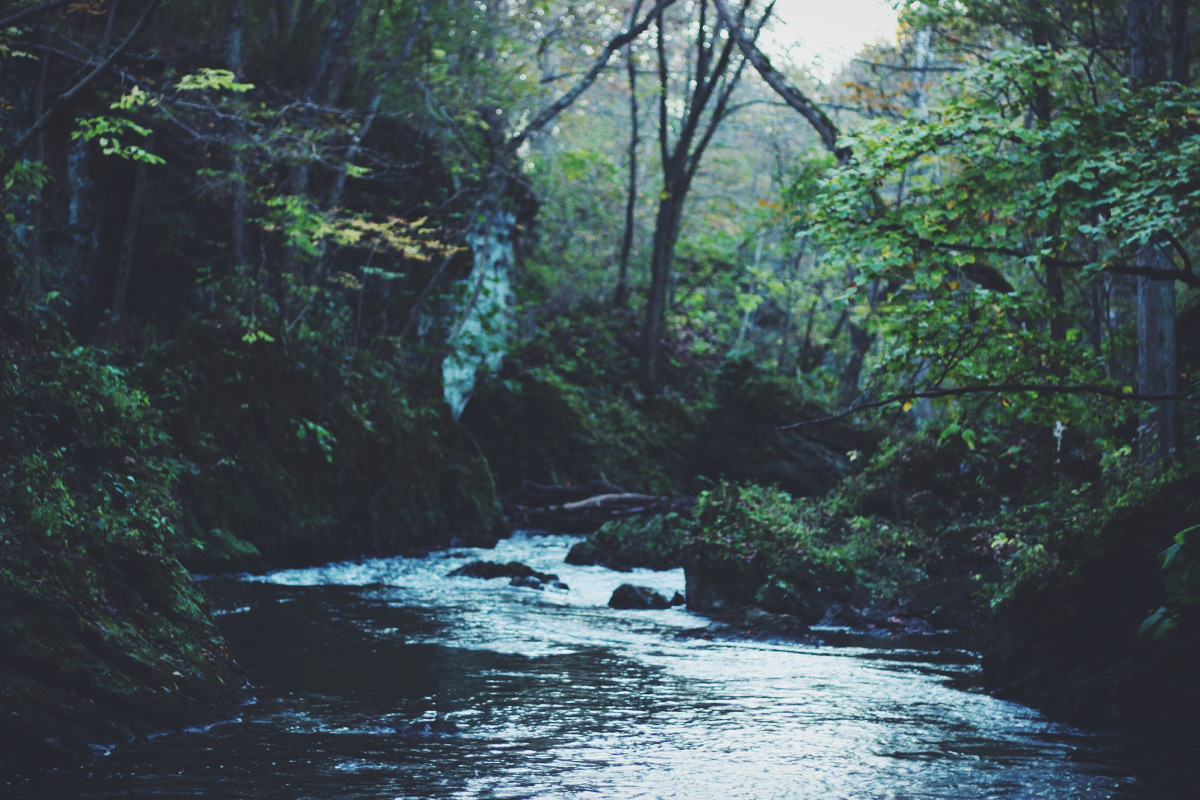
\includegraphics[width=\linewidth]{stream}
% \caption{Legend (350 words max). Example legend text.}
% \label{fig:stream}
% \end{figure}


% \begin{table}[ht]
% \centering
% \begin{tabular}{|l|l|l|}
% \hline
% Condition & n & p \\
% \hline
% A & 5 & 0.1 \\
% \hline
% B & 10 & 0.01 \\
% \hline
% \end{tabular}
% \caption{\label{tab:example}Legend (350 words max). Example legend text.}
% \end{table}

\end{document}
